\documentclass[a4paper,10pt]{report}
\usepackage[utf8]{inputenc}
\usepackage{blindtext}
\usepackage{hyperref}

\usepackage{graphicx}
\usepackage{polski}
\usepackage[utf8]{inputenc}
\usepackage{amssymb, amsmath}
\usepackage[top=2in, bottom=1.5in, left=1in, right=1in]{geometry}


\title{Zarządzanie}
\author{Jakub Pyszka}
\begin{document}

\maketitle
\tableofcontents{}

\chapter{Temat 1}

\section{24 II 2015r. (Górski)}

Zarządzanie obejmuje kształtowanie produltywnej współpracy jednostek i frup wewnątrz organizacji oraz dopasowanie tych wysiłków do wymagan formułowanych przez jej otoczenie, z którym organizacja musi dokonywać WYMIANY jeśli chce przetrwać. \\
\indent Kwintesencją roli menedżera jest kierowanie tego typy wymianami ze stronami znajdującymi się w organizacji i poza nią, by mogła ona trwać w dłuższej perspektywie czasu.\\ \\

/ZARZĄDZANIE = (?) ORGANIZOWANIE PRACY/ \\
No nie... zarządzanie to więcej niż organizacja pracy. 



\section{26 II 2015r. (Opolski)}
Podejście systemowe i holistyczne: \\
(holizm -- patrzenie całościowe)
Organizacja to system. Elementy mające funkcje. Jest powiązanie między elementami z elementem organizującym. Elementy pasują do siebie.\\ 
Pytania o autonomię poszczególnych części (zależy od organu sterującego np. zarząd). \\
Organizacja jest otwarta względem otoczenia. Coś pobiera z otoczenia, a coś oddaje. Bierze (kupuje) zasoby. Oddaje (sprzedaje) produkt. Ma zasilenie (środki) na kolejne zasoby. \\
Symptomem zamykania się organizacji na otoczenie jest spadek rotacji zapasów. \\
Podejście BSC (zbilansowana karta wyników). Autorzy Kapplan, Norton. Pokazuje cztery perspektywy w organizacji. Perspektywy finansowa, klienta, procesów wewnętrznych, rozwoju. Nie można powiedzieć, że organizacja jest nastawiona na jedną z tych perspektyw. Organizacja zmierza do sukcesu. Non-profit inaczej definiuje sukces niż for profit itp. Organizacja musi łączyć te perspektywy w harmonijny sposób. Do każdej perspektywy musimy określić jakiś cel. \\

\noindent Zapamiętać:
\begin{itemize}
	\item Holistyka
	\item System jako system otwarty
	\item Turbulencja
	\item Zbilansowana karta wyników
\end{itemize}

\noindent Relacja między ekonomią a zarządzaniem

\begin{itemize}
	\item Planowanie 
	\begin{itemize}
		\item Apekty ekonomiczne: zysk (przeznaczany na konsumpcje lub ekumulacje), wartość firmy, Inwestycje (dwa aspekty: wielkość zwrotu i czas), zapasy, źródła zaopatrzenia, kapitał -- obcy lub własny.
		\item Aspekty zarządcze: Planowanie operacyjne lub strategiczne. Budowa strategii. Wybór (efektywnościowy). Aspekty wewnętrzne i zewnętrzne -- kwestia konkurencyjności.
		\item Teorie ekonomiczne: Strategia, teoria gier, finanse + rachonkowość
	\end{itemize}
	\item Kontrolowanie
	\begin{itemize}
		\item Aspekty ekonomiczne: Koszty i dynamika kosztów. Rentowność. Ryzyko.
		\item Aspekty zarządcze. Rola kontroli, organizacja kontroli, miejsce kontroli w systemie zarządzania, decyzje pokontrolne, 
		\item teorie ekonomiczne: teoria agencji (pryncypał -- agent), teoria kosztów transakcyjncych
	\end{itemize}
	\item Informowanie
	\begin{itemize}
		\item Aspekty ekonomiczne: rodzaj mierników ekonomicznych, które biorę pod uwagę (informowanie o wyniku firmy). Interpretacja mierników. 
		\item Aspekty zarządcze: Adresat informacji, dostęp do informacji, kodowanie informacji, treść informacji, CSR -- corporate social responsibility
		\item Teorie ekonomiczne: Teoria sygnalizacji, 
	\end{itemize}
	\item Kierowanie
	\begin{itemize}
		\item Aspekty ekonomiczne: Koszty pracy, rynek pracy (popyt, podaz), relacja kosztów stałych do zmiennych, ryzyko operacyjne (ryzyko popełniania błędów przez pracowników [świadomych lub nie]), inwestycje w jakość z punktu widzenia kosztów i korzyści.
		\item Aspekty zarządcze:
		\item Teorie ekonomiczne: teoria rynku pracy, signaling.
	\end{itemize}
	\item Motywowanie
	\begin{itemize}
		\item Aspekty ekonomiczne: Rynek pracy (dostępność siły roboczej), rachunek kosztów stałych do kosztów zmiennych (czy zatrudniać na stałe czy do projektóœ), model konsumpcji (indywidualna, zbiorowa [dać mu samochód lub benefit), finanse gospodarstw domowych (oszczędności i zadłużenie)
		\item Aspekty zarządcze: Bodźce -- kary i nagrody (wywarzenie proporcji), model przywództwa (oparty na władzy, formalnych aspektach czy respekt rzeczywisty), kultura organizacyjna (normy, wartości, przekonania, preferencje), HRM (human resource management) -- szkolenia, rekrutacja, selekcja.
		\item Teorie ekonomiczne: teoria agencji i teoria kosztów transakcyjnych
	\end{itemize}
	\item Decydowanie
	\begin{itemize}
		\item Aspekty ekonomiczne: podział zysku, wielkość dywidendy, kierunek rowoju firmy, rozwój wewnętrzny -- organiczny, rozwój zewnętrzny -- M\&A, pomiar ryzyka np. VAR
		\item Aspekty zarządzcze: relacje inwestorskie (nawiązywanie kontaktór, wpółpracy z inwestorami), zarządzanie zmianą, zarządzanie konfliktami, negocjacje, percepcja ryzyka,  
		\item Teorie ekonomiczne: signaling
	\end{itemize}
\end{itemize}

Obszary zainteresowania:
\begin{itemize}
	\item Finanse:
	\begin{itemize}
		\item perpektywa rozwoju
		\item dezycje o zmianach
	\end{itemize}
	\item Wiedza z rachunkowści -- decyzje cenowe, rachunek kosztów, marża.
	\item Strategia
	\item Marketing -- rynek, klient, popyt, kanały komunikacji.
	\item Bankowość -- koszt kapitału obcego, dostępność kredytu, ryzyko kredytu, dostępne produkty bankowe
	\item Wiedza psychologiczna (społeczna) -- jak wydawać polecenia, jak silne muszą być kary i nagrody, jak reaguję sie wobec grupy, jak reagują grupy, jak się pracuje w zespole
	\item Makroekonomia -- polityka pieniężna, tempo wzrostu PKB, poziom konsumpcji, preferencje konsumpcje, aspekty globalne: konkurencja globalna itp.
\end{itemize}

Podsumowanie w paru słowach. 
W ekonomii występuje analiza costs--benefit. Koszt i korzyść ma również wymiar psychologiczny, a nie tylko finansowy. 


\section{3 III 2015r. (Górski)}

Organizacja \\

Efektywność, skuteczność i użyteczność zarządzania. Efektywność to nie skuteczność. Firma mająca zysk, ale nie mająca płynności jest skuteczna, ale nie jest efektywna. \\
\begin{itemize}
	\item Efektywność (efficiency): Nakłady (inputs) -- produkty (outputs)
	\item Skuteczność (effectiveness): Cele -- Rezultaty (outcomes) i Oddziaływanie (impact)
	\item Użyteczność (utility): Potrzeby -- Oddziaływanie (impact)
\end{itemize}

\indent Aby być skutecznym potrzebujemy zdefiniować cel i rezultaty. Często patrzymy tylko i wyłącznie na rezultaty, ale to błąd. Miara skuteczności jest miarą relatywną, między celem, a rezultatem (adekwatność). Problem nieskuteczności bardzo często pociąga za sobą nieefektywność organizacji. Warto zdefiniować misję organizacji, aby zakotwiczyć działalność w szerszym kontekście. Misja może wynikać np. z potrzeb społecznych. Misja uwiarygadnia działania organizacji. \\


\newtheorem{Organizacja 1}{Organizacja}
\begin{Organizacja 1}
Organizacja to pewien rodzaj całości której wszystkie składniki współprzyczyniającą się do powodzenia całości. T. Kotarbiński.
\end{Organizacja 1}

\newtheorem{Organizacja 2}{Organizacja}
\begin{Organizacja 2}
Organizacja to taka całość, która przyczynia się do powodzenia swych części. A.K. Koźmiński, K. Obłój
\end{Organizacja 2}

Firma jest elementem większej organizacji (rynku, społeczeństwa). Firma jest wtedy jednostką w ramach tej organizacji.\\

Analogie organizacji (metafory organizacyjne) \\
$[$Morgan, G. (1997). Obrazy organizacji. Warszawa: PWN$]$
\begin{itemize}
	\item Organizacja jako maszyna
	\begin{itemize}
		\item Organizacja doskonale sprawna, złożona z idealnie dopasownych do  siebie elementów koordynowanych za pomocą racjonalnie realizowanych funkcji kierowniczych.
		\item Założenia 
		\begin{itemize}
			\item Organizajca jest instrumentem osiągania zadanego z zewnątrz, precyzyjnie sformułowanego celu. 
			\begin{itemize}
				\item Organizacja nie jest autonomiczna
				\item jest pewna siła sprawcza
				\item organiacja jest zaprojektowana raz
				\item łatwo obalić w dzisiejszych (dynamicznych) czasach			
			\end{itemize}
			\item Uczestnicy organizacji są jedynie powolnymi narzędziami osiągania celu (specjalizacja ekstremalna)
			\item Kierownik ma jednostronne prawo do wydawania poleceń podwładnym i egzekwowania ich posłuszeństwa (zhierarchizowana struktura władzy).
			\begin{itemize}
				\item Ciągle istnieją takie firmy, ale bardzo często nie są to najlepsze organizacje
			\end{itemize}
			\item Podstawowe uprawnienia decyzyjne są zlokalizowane na najwyższym szczeblu hierarchii organizacyjnej (władza i informacje są scentralizowane).
		\end{itemize}
		\item Cechy
		\begin{itemize}
			\item suma sprawnych i niezawodnych elementów będzie tworzyła sprawną całość
			\item minimalizacja tarcia organizacyjnego przez planowanie, rozkazywanie, koordynację, kontrole
			\item systemy motywacyjne: $"$kij i marchewka$"$
		\end{itemize}
		\item Podsumowanie
		\begin{itemize}
			\item Organizacja jako zespół dobrze ustrukturyzowanych części o ściśle określonyc rolach i zadaniach
			\item Nacisk na sprawność, wydajność. Ludzie widzeni jako elemntu mechanizmu, działające w sposób określony przez ich zadania
		\end{itemize}
	\end{itemize}
	\item Organizacja jako organizm
	\begin{itemize}
		\item Analogia ta porównuje zespoły pracownicze i całe organizacje do żywych organizmów, eksponując element przetrwania i dostosowania się organizacji do zmian zewnętrznych, a nie optymalizacji i idelanej koordynacji
		\item Model organizacji się zmienia, bo otoczenie się zmienia (prawo, klienci, rynek) -- ewolucja organizacji
		\item Zupełnia inna wizja organizacji w porównaniu do organizacji jako maszyny
		\item obsesja działania jako źródło sukcesu
		\item Założenia
		\begin{itemize}
			\item Organizacja jest złożoną całością (systemem) pozostającą w stałych relacjach z otoczeniem
			\begin{itemize}
				\item zmiany ex post -- łatwe, bo śledzimy lepszych konkurentów
				\item ex ante -- dużo trudniejsze
			\end{itemize}
			\item Nadrzędnym celem organizacji jest przetrwanie
			\begin{itemize}
				\item Obzary ryzyka
				\item oczekiwania klientów w przyszłości (np. w perspektywie 10 lat)
				\item wygrywają firmy wyprzedzające przyszłość (tworzące przyszłość)
			\end{itemize}
			\item Naturalnym i pożądanym stanem organizacji jest stan równowagi (homeostazy) i umiejętności przywracania tej równowagi
			\begin{itemize}
				\item organizacji musi pozostawać we względnej równowadze, ale nie statycznej. When you stop -- you die.
			\end{itemize}
			\item Zmiana organizacji jest abo wynikiem adaptacji do zmienionych wymagań otoczenia, albo naturalnym efektem cyklu życia organizacji (bierna adaptacja)
		\end{itemize}
		\item Cechy
		\begin{itemize}
			\item musi się zmieniać
			\item posiada nadmiar organizacyjny (luz organizacyjny, organizational slack) służący do przetrwania ($"$sadło$"$ organizacji -- przerosty, luzy czasowe)
			\item znaczenie informacji (przepływy informacyjne)
			\item analiza ścieżki krytycznej (PERT -- Program Evaluation and Review Technique -- stochastyczna metoda planowania i kontroli projektu, wykorzystująca programowanie sieciowe, stosowana w zarządzaniu projektami)
			\item swoboda działania podsystemów
			\item wzrost zróżnicowany
			\item świat organizmu to świat harmonii -- motywacja
		\end{itemize}
		\item Podsumowanie
		\begin{itemize}
			\item Organizacja jako był podatny na upływ czasu (narodziny, rozwój, dojrzałość, starzenie się, śmierć), działający w otoczeniu i od niego zależny
			\item Nacisk na otoczenie. Organizacja to całość, elastyczne dostosowywanie się do otoczenia, zaspokajanie własnych potrzeb.
		\end{itemize}
	\end{itemize}
	\item Organizacja jako gra
	\begin{itemize}
		\item Jest to podejście systemowe, w którym zwraca się uwagę na powiązanie organizacji z otoczeniem oraz na sprzeżenia zwrotne między poszczególnymi procesami i podsystemami wewnątrz organizacji. 
		\item Zasadniczym czynnikiem integracji organizacyhnej są reguły gry.
		\item Z kim gramy?
		\begin{itemize}
			\item z dostawcą
			\item z klientem
		\end{itemize}
		\item Instrumenty gry:
		\begin{itemize}
			\item cena
			\item jakość
			\item ...
		\end{itemize}
		\item Gra na zewnątrz, ale też wewnątrz (pracownicy -- przełożeni: teoria agencji)
		\item Założenia:
		\begin{itemize}
			\item Organizacja jest sztuczną konstrukcją społeczną, którą tworzą autonomiczni uczestnicy
			\item Cele uczestników organizacji są różne i niesprowadzalne do wspólnego mianownika
			\item Zasadniczym cznnikiem integracji organizacyjnej są reguły gry, w ramach krótych autoomiczni gracze wykorzystają swoje zasoby i tworzą strategie działania
			\item Konflikty i zmiana stanowią siłe motoryczne rozwoju organizacji
		\end{itemize}
		\item Cechy:
		\begin{itemize}
			\item różna racjonalność działania aktorów -- graczy [człowiek działa racjonalnie, ale w sposób ograniczony swoimi zmysłami, wiedzą itp.]
			\item możliwość wystąpienia konfliktów i sprzeczności jako cechy gry
			\item pojęcie racjonalności (ekonomia neoinstytucjonalna i industrail economics, ekonomia behawioralna) 
		\end{itemize}
	\end{itemize}
	\item Organizacja jako mózg
	\begin{itemize}
		\item Systemy przetwarzające informacje i uczące się. Polepsza jakość organizowania, w taki sposób, aby wspierać działania elastyczne i twórcze.
		\item Organizacja jest instytucją (samo)doskonalącą się		
		\item Podsumowanie
		\begin{itemize}
			\item Organizacja jako twór rozumie działający i uczący się
			\item Nacisk na zdolność uczenia się.. Ludzie jako naważniejszy zasów w organizacji
		\end{itemize}
	\end{itemize}
	\item Organizacja jako kultura
	\begin{itemize}
		\item Organizacja jest zjawiskiem kulturowym zmieniającym się zgodnie ze stadium rozwoju społecznego.
		\item Kultura -- zespół norm, zachowań, tradycji
		\item Podsumowanie
		\begin{itemize}
			\item Organizacja jako rodzaj symbolicznego sposobu porozumiewania się i działania, odmiennego od działania innych
			\item Nacisk na indywidualny charakter organizacji na zewnątrz i jednoznaczne, wspólne wartości oraz postawy wewnątrz
		\end{itemize}
	\end{itemize}
	\item Organizacja jako system polityczny
	\begin{itemize}
		\item Metafora eksponująca stusunki władzy w organizacji i wynikające z nich konflikty
		\item Organizacja musi znaleźć sposoby tworzenia ładu i wspólnego kierunku działania między ludźmi o potencjalnie sprzecznych interesach.
		\item Podsumowanie
		\begin{itemize}
			\item Organizacja jako sięc ludzi działających razem, by osiągnąć indywidualne cele
			\item Nacisk na władzę, jako sposób reagowania na konflikty oraz zapobiegania przecznym działaniom
		\end{itemize}
	\end{itemize}
	\item Organizacja jako psychiczne więzienie
	\begin{itemize}
		\item Podejście koncentruje uwagę na ograniczeniach i konflikcie między potrzebami jednostki a regułami organizacji.		
		\item Podsumowanie
		\begin{itemize}
			\item Organizacja jako sposób stereotypowego podejścia do zjawisk, organiczająca indywidualne cechy
			\item Nacisk na ograniczanie wolności jednostki, poprzez narzucanie stereotypowych potaw i zachowań
		\end{itemize}
	\end{itemize}
	\item Organizacja jako narzędzie dominacji
	\begin{itemize}
		\item Cechą organizacji jest połączenie osiągnięć i wyzysku.
		\item Podsumowanie
		\begin{itemize}
			\item Organizacja jako sposób wyzysku, stale kontrolująca postępowanie i postawy ludzi z nią związanych
			\item Nacisk na kontrolę i dominację organizacji nad ludźmi, wykorzytywanie ich możliwości do osiągania najlepszych wyników.
		\end{itemize}
	\end{itemize}
\end{itemize}

\section{5 III 2015 (Opolski)}

Offtop: \\
Od czego zależy sukces? Pasja. Instrument do poszukiwania wiedzy, do chęci poszukiwania do działania. Wizja. Wsparcie. Budowanie relacji (network). \\

(dokńczenie wykładu o metaforach [patrze Górski]\\

Podejści systemowe:\\
Szerokie widzenie analizowanego problemu, traktowanie każdej organizacji jako całości, której wszystkie problemy powinny być rozwiązywane globalnie.\\

Ojcowie podejścia ystemowego: Ludwig von Bertalanffy, Norbwert Wiener\\

System otwarty, w których wejście energii i prekształcenie wyjścia w następne wejście energetyczne opira się na transakcji między organizacją a jej otoczeniem. \\
Cechy sytemu otwartego (katz, Kahn):
\begin{itemize}
	\item Pobieranie energii
	\item Przejścia (przetwarzanie)
	\item WYjścia
	\item Systemy jako cykle zdarzeń (struktura)
	\item Negatywna entropia (warunkiem przetrwania systemów społecznych jest działanie w kierunku zatrzymania procesu entropii -- negentropia) -- chcemy zachamować proces rozpadu, chcemy uporządkowania w ramach organizacji
	\item Wejścia informacyjne, proces kodowania
	\item Stan ustalony i komeostaza dynamiczna (proces zmiany rezerwy, fuzji i przejęcia, wzrost, ekspansja)
	\item Zróżnicowanie (specjalizacja)
	\item Ekwifinalność (system może osiągnąc ten sam stan finalny przy różnych warunkowych wstępnych i za pomocą różnych sposobów -- von Bertalonffy)
\end{itemize}

System społeczny, tzn. skłąda się z modelowanych działań szeregu jednostek (są one powtarzalne, względnie stałe oraz powiązane w czasie i przestrzni). 
Jest jakaś architektura w tych działaniach.\\ 
Modeluje się działania ludzi -- potrzebna do kontroli, przewidywania zachowań, daje rodzaj miary między tym jakie są wyniki, a jakie chcielibyśmy \\
surowce i praca ludzka = wejście energetyczne \\
modelowanie działania produkcyjne = przekstzałcanie energii
ukończony prdukt => wyjście\\

Zapamiętać:\\
system otwarty\\
ekwifinalność\\

\section{10 III 2015 (Górski)}
Charakterystyczne cechy organizacji i jej podsystemy (Katz, Kahn):\\
Systemy społeczne charkteryzują się dużą zmiennością i z łatwością można je projektować dla różnych celów o szerokim zakresie, a każdy powstały już system może nabyć nowe i odmienne od założonych funkcje podczas swojego istnienia. (Śmierć i narodziny organizacji)\\
Organizacja ucząca się. Co to znaczy? organizacja rozwija się i ma pamięć. SUkces nie jest zależny od konkretnego świetnego pracownika i jak odejdzie to organizacja zawodzi. Organizacja zna źródła sukcesu tego pracownika i pamięta to i może przekazać wiedze dalej.\\

Czynniki redukujące zmienność w systemie:
\begin{itemize}
	\item naciski środowiska (dziś np. ekologia)
	\item podzielone wartości i oczekiwanie (style kierowania)
	\item wprowadzenie przepisów (nadzór i kontrola)
\end{itemize}

Trzy podstawy integracji systemu
\begin{itemize}
	\item Role = opis specyficznych (wystandaryzowanych) form zachowań związanych z danymi zadaniami (wywodzi sie z wymagań zadania)
	\begin{itemize}
		\item powinny być dobrze wyspecyfikowane
		\item każdy powinień rozumieć swoją rolę w organizacji (jeśli nie --> główny powód wypalenia zawodowego)
	\end{itemize}
	\item Normy = ogólne oczekiwania o charakterze zadań odnoszących się do wszystkich osób pełniących role w systemie (podsystemowe)
	\begin{itemize}
		\item wchodzi tu w grę m.in. misja firmy
		\item integracja ludzi na poziomie wpólnych przekonań o organizacji
	\end{itemize}
	\item Wartości = bardziej ogólne, ideologiczne uzasadnienia i dążenia
	\begin{itemize}
		\item Aksjologia
		\item w to wierzymy, to robimy
		\item przykład: firma przechodzi duży kryzys, a mimo to rezygnuje z połowy wynagrodzenia, bo wierze w firmę, markę itp.
		\item Przekonanie: jakość jest najważniejsza, rzetelność jest najważniejsza
	\end{itemize}
\end{itemize}

\noindent Typy podsytemów w ogranizacji\\
\begin{itemize}
	\item Podsystemy produkcyjne (techniczne)
	\begin{itemize}
		\item obejmują procesy przejścia, tj. przetwarzanie energii lub informacji (czyli cykl działalnośći produkcyjnej)
	\end{itemize}
	\item Podsytemy wspierające
	\begin{itemize}
		\item są to te struktury, które dokonują wymiany z otoczeniem dostarczając wejść, lokując produkty lub wspomagając te procesy (pobierają materiały, które poddawane są obróbce i eksportują produkt)
		\item zbyt, zapoatrzenie, marketing (PR), rada nadzorcza
	\end{itemize}
	\item podsystemy scalające
	\begin{itemize}
		\item modelowane zachowania ludzkie (rekrutacja, selekcja, motywacja)
		\item przywiązują one ludzi do systemu tworząc z nich funkcjonalne części
		\item główne podstruktury scalające to SYSTEM NAGRÓD I KAR.
	\end{itemize}
	\item podsystemy adaptacyjne
	\begin{itemize}
		\item zadaniem jest wyczuwanie odpowiednich zmian w świecie zewnętrznym i objaśnianie znaczenia tych zmian dla organizacji (R\&D, badania rynku, strategie)
	\end{itemize}
	\item podsystemy kierownicze
	\begin{itemize}
		\item kontrola i koordynacja = REGULACJA
		\item struktura zwierzchnictwa
		\item forma podejmowania decyzji
	\end{itemize}
\end{itemize}

\noindent Podsystemy organizacji i dylematy z nich wynikające:
\begin{itemize}
	\item podsystem produkcyjny
	\begin{itemize}
		\item chociaż sprawność techniczna powstaje jako naturalna wartość w systemie produkcji, nie gwarantuje ona efektywności całej organizacji. ("pracownicy sprawni technicznie mogą być negatywnie ustosunkowanie do przepisów organizacji")
	\end{itemize} 
	\item Podsystem scalający
	\begin{itemize}
		\item formalizacja (uniformizacja) (nastawiony na utrzymanie stabilności i predyktywności sytemu)
		\item instytucjonalizacja wszystkich zachowań organizacji
		\item Rytualizacja ("Jeśli masz coś do powiedzenia, napisz to. Pamiętaj, że rozmowy nie można ciągnąc do kartotek")
		\item konserwatyzm
		\item zabija kreatywnośc w organizacji, organizacja nie ma być skostniała... ma być stabilna, ale nie skostaniała
	\end{itemize}
	\item Podsystem wspierający (graniczne)
	\begin{itemize}
		\item presja na klienta, a nie na zmienę wewnątrz organizacji
		\begin{itemize}
			\item Klienci się zmieniają...
			\item zadowolenie klienta -- NIE za wszelką cenę
		\end{itemize}
	\end{itemize}
	\item podsystem adaptacyjny
	\begin{itemize}
		\item zmierzanie do osiągnięcia stałości (skierowany na zewnątrz) środowiska próbując poddać świat zewnętrzny sowjej kontroli (reklama + PR)
		\item kształtowanie gustów tak, aby dopasować je do produktu ("klient jest głupi")
		\begin{itemize}
			\item silny może tak robić, choć nie zawsze
		\end{itemize}
		\item Uwaga: Czy organizacja chce się zmieniać???
		\begin{itemize}
			\item w naturze ludzkiej jest to, żeby się nie zmieniać
		\end{itemize}
	\end{itemize}
	\item podsystem kierowniczy
	\begin{itemize}
		\item kierownistwo może znajdować się pod większym wpływem jednego z podsystemów lub też (częściej) mające pochodzenie struktury nieformalnej (z jakiej struktury się wywodzi).
		\item organizacja może faworyzować pewne elemnty w organizacji poprzez osobę menadżera -- duże ryzyko
	\end{itemize}
\end{itemize}

\noindent Podejście sytemowe w diagnostyce organizacji -- zastosowanie SSM
\begin{itemize}
	\item Podsystem zarządzania
	\item Podsystem społęczno-kulturowy
	\item podsystme technologiczny
	\item podssytem procesowo funkcjonalny
	\item podsystem strategii i celów
\end{itemize}

\noindent Cykl życia organizacji:
\begin{itemize}
	\item 1 faza -- inicjacja
	\item 2 faza -- ekspansja
	\item 3 faza -- dojrzałość
	\item 4 faza -- dryfowanie
	\item 5 faza -- załamanie
	\item 6 faza -- upadek
\end{itemize}

\noindent Cykl życia organizacji
\begin{itemize}
	\item Etap I: rozwój przez kreatywność
	\begin{itemize}
		\item kryzys przywództwa
	\end{itemize}
	\item Etap II: rozwój przez wytyczne
	\begin{itemize}
		\item kryzys autonomii
	\end{itemize}
	\item Etap III: rozwój przez delegowanie uprawnień
	\begin{itemize}
		\item Kryzys kontroli
	\end{itemize}
	\item Etap IV: rozwój przez koordynacji
	\begin{itemize}
		\item kryzys biurokracji (red tape)
		\item za dużo zasobów jest marnowanych przez zajmowanie się organizcją przez samą organizację
	\end{itemize}
	\item Etap V: rozwój przez współpracę -- kultura korporacyjna itp.
	\begin{itemize}
		\item kryzys?
	\end{itemize}
\end{itemize}

\noindent Cykl życia organizacji -- koncepcja L.E. Greinera
\begin{itemize}
	\item Faza 1: Kreatywność 
	\begin{itemize}
		\item Kryzys przywództwa (Leadership)
	\end{itemize}
	\item Faza 2: Kierunkowanie -- (określenie kierunkóœ rozwoju i precyzyjne sformułowanie cełow. Budowanie struktur organizacyjnych. Formalizacja / centralizacja
	\begin{itemize}
		\item Kryzys autonomii (Autonomy)
	\end{itemize}
	\item Faza 3: Decentralizacja -- delegacja uprawnień, ale zwiększanie zakresu kontroli, komunikowanie sformalizowane, nadmiar autonomii
	\begin{itemize}
		\item Kryzys sterowania (Control)
	\end{itemize}
	\item Faza 4: Koordynacja -- organiczenie autonomii poprzez tworzenie grup zorientowanych na produkt/rynek/zysk
	\begin{itemize}
		\item Kryzys złożoności (Red tape)
	\end{itemize}
	\item Faza 5: współpraca i współodpowiedzialność
	\begin{itemize}
		\item Kryzys?
	\end{itemize}
\end{itemize}

Z tej teorii wynika, że menadżer jest mózgiem organizacji, któ©y kreauje jej samoświadomość

\noindent Cykl życia organizacji -- koncpecja Quinna, Camerona, ROhrbauhna
\begin{itemize}
	\item Faza 1: przedsiębiorczości ("JA")
	\begin{itemize}
		\item uzyskanie dostępu do zasobów (walka)
		\item mnogość pomysłów
		\item działania przedsiębirocze
		\item mało planowania i koodynacji
		\item utworzenie niszy (wejście w niszę)
		\item INNOWACYJNOŚĆ -- ENKLAWA -- KREATYWNOŚĆ
	\end{itemize}
	\item Faza 2: kolektywności ("MY")
	\begin{itemize}
		\item nieformalne komunikowanie i struktura
		\item duża koletywność
		\item praca bez liczenia się z czasem
		\item poczucie misji i duże zaangażowanie
		\item WYSOKA SPOISTOŚĆ + ZAANAGAŻOWANIE
	\end{itemize}
	\item Faza 3: formalizacji i sterowanie
	\begin{itemize}
		\item formalizacja reguł i zasad
		\item stabilna i formalna struktura
		\item nacisk na wydajność i utrzymanie sprawności
		\item konserwatyzm (niechęc do zmian)
		\item instytucjonalizacja procedur działania
		\item STABILNOŚĆ + INSTYTUCJONALIZACJA
	\end{itemize}
	\item Faza 4: przekształcenia struktur
	\begin{itemize}
		\item przekształcenie struktury
		\item decentralizacja
		\item rozszerzenie zakresu działania
		\item odnowa
		\item ELASTYCZNOŚĆ + STEROWNOŚĆ + PRZEŁAMANIE RUTYNY I INERCJI
	\end{itemize}
\end{itemize}

Między fazą 2 i 3 jest OGROMNA zmiana widzenia organizacji. W fazie 3 organizacja narzuca zasady, a we wcześniejszy "ja" lub "my" narzucamy firmie zasady.

\section{12 III 2015 (Opolski)}

Wartość gratyfikacyjna -- siła motywacyjna i prawdopodobieństwo osiągnięcia gratyfikacji.\\


\noindent Metafory struktur organizacyjnych (T. Lambert "Problemy zarządzania 50 praktycznych modeli rowiązań", Dom Wydawniczy ABC, W-wa 1999)
\begin{itemize}
	\item Autokracja -- czyli pajęczyna; wszystkie linie komunikacji prowadzą bezpośrednio lub pośrednio do przedsiębiorcy autokraty -- pająka. 
	\begin{itemize}
		\item wada: wszystko się opiera na jednej osobie, może występować spaczona wizja
		\item zaleta: szybki proces decyzyjny, jednolita wizja, brak dyfuzji odpowiedzialności
	\end{itemize}
	\item Biurokracja -- grecka świątynia, w której zespół kierowniczy zasiada na frontonie, a pozostała część struktury mieści się w poszczególnych kolumnach. (Komunikacja pioniowa między kolumnami, a pozioma tylko w warstwie kierowniczej).
	\begin{itemize}
		\item wada: kosztowny proces decyzyjny
		\item zaleta: jasny i ustalony podział wg odpowiedzialności, nie wchodzi sobie nawzajem w kompentencje
	\end{itemize}
	\item Organizacja macierzowa -- sieć, komunikacja przebiega w zależności od potrzeby, we wszystkich kierunkach.
	\begin{itemize}
		\item zaleta: dobry przepływ informacji, komunikacja (przede wszystkim) pozioma, liczą się kompetencje w ramach projektu
		\item wada: groźba chaosu, groźba podwójnej odpowiedzialności (kogo słuchać, projekt ma być na czas, czy ma być porządnie zrobiony), groźba doboru ludzi do projektu o niewłaściwych kompentencjach
	\end{itemize}
	\item Koniczynka
	\begin{itemize}
		\item jeden listek = najważniejsi pracownicy, trzon
		\item drugi = zewnętrzni dostawcy usług
		\item trzeci = "elastyczna" siła robocza, zmienialni łatwo zastępowalni, ale dostępni (dyspozycyjni)
		\item czwarty = "usługi wewnętrzne" zlecane na zewnątrz -- outsourcing (za Charles Handy)
	\end{itemize}
\end{itemize}

\noindent Wzory zachowań organizacyjnych wg Ansoffa (Ojca szkoły zarządzania strategicznego)
\begin{itemize}
	\item Spoglądając wstecz organizacje preferują wybory, które odniosły sukces w przeszłości (odejśce od precedensów jest podejrzane i należy go unikać).
	\begin{itemize}
		\item w krótkim okresie może przynieść sukces
		\item "Uderz jeszcze raz w to samo miejsce"
	\end{itemize}
	\item Organizacje są przygotowane do odejścia od przeszłosci na tyle, na ile to odejście nie różni się specjalnie przeszłych doświadczeń.
	\begin{itemize}
		\item lekkie rozluźnienie poprzedniego punktu
		\item "Jesteśmy przygotowani toczyć się dopiero, gdy nas popchną"
	\end{itemize}
	\item Organizacje ekstrapolując w przyszłość starają się przewidzieć zagrożenie i możłiwości. Ich stosunek do otoczenia ma aktywny charakter. Zamiast oczekiwać aż je ogarną nowe okoliczności same poszukują nowych kierunków działania. Jednakże wartość swoich opcji sprawdzają za pomocą tradycyjnych i sprawdzonych miar i sposobu percepcji i modeli rzeczywistości. Wybór musi być przedłużeniem poprzedniego doświadczenia.
	\item Organizajce wychodzą poza ekstrapolację na spotkanie nowych światów i rzeczywistości, poszukują zarówno nowatorstwa, jak i nie znanych możliwości. Zjawiska niezgodne z doświadczeniem nie są odrzucane
	\item Twórcy informacji są także twórcami działań -- "Wymyśl przyszłość".
	\begin{itemize}
		\item firmy poprzez marketing uświadamiają potrzeby
		\item iPhone, walkman, Polaroid
	\end{itemize}
\end{itemize}


\noindent Klasyfikacja rodzajów decyzji: 3S (Strategy, Structure, Systems)
\begin{itemize}
	\item Strategiczne (produkt -- rynek)
	\item Administracyjne (organizacja, alokacja zasobów)
	\item Operacyjne (budżetowanie, bieżace kierowanie)
	\begin{itemize}
		\item 3P
	\end{itemize}
\end{itemize}

\noindent Komponenty strategii wg Ansoffa
\begin{itemize}
	\item Zakres produkt rynek
	\begin{itemize}
		\item Peters, Waterman, In search of excellence: "stick to the knitting" (stay with the busines that you know)
	\end{itemize}
	\item Wektor wzrostu
	\begin{itemize}
		\item w którym kierunku wzrost
	\end{itemize}
	\item Przewaga konkurencyjna
	\item Michael Porter
	\begin{itemize}
		\item Synergia: "$2 + 2 = 5$"
		\item Testowanie, jak okazje "pasują" do kluczowych przewag konkurencyjnych firmy
	\end{itemize}
\end{itemize}

\chapter{
Temat 2 Przedsiębiorstwo jako specyficzna forma organizacji: cele, formy, zasoby}

\section{12 III 2015 (Opolski)}

\noindent Przedsiębiorstwo to podmiot gospodarczy prowadzący na własny rachnuek działalność produkcjyną lub usługową w celu osiągnięcia określonych korzyści.

\begin{itemize}
	\item Podmiot gospodarczy: forma prawna, zakres działań, struktura organizacyjna
	\item na własny rachunek: ponosi odpowiedzialność finansową
	\item w celu osiągnięcia określonych korzyści: dywidenda, intelektualna korzyść, itd. itp.
\end{itemize}

\noindent Koncepcja całości przedsiębiorstwa
\begin{itemize}
	\item Czynniki sytuacyjne
	\begin{itemize}
		\item Czym jest przedsiębiorstwo i kim są ludzie, którzy o nim decydują (status, typ własności, kontrakty menedżerskie, uprwanienia decyzyjne, aktywa/kapitał, obrót, zatrudnienie, źródła finansowania, lokalizacja i własność gruntów itp.)
	\end{itemize}
	\item Czynniki działalności
	\begin{itemize}
		\item co przedsiębiorstwo robi (no. typ produkcji, metody kontroli, procedury, prognozy, informacje, technologia, kadry).
	\end{itemize}
	\item Czynniki osiągnięć
	\begin{itemize}
		\item Jak dobrze przedsiębiorstwo prowadzi swoją działalność (firma i rynek)
	\end{itemize}
	\item Czynniki strukturalne
	\begin{itemize}
		\item Jak przedsiębirostw jest zorganizowane dla prowadzenia sowjej działalności (formalny schemat organizacyjny, autorytety, kultura, rozwój kadr)
	\end{itemize}
\end{itemize}

\section{17 III 2015 (Górski)}

\noindent Cechy przedsiębiorstwa 

\begin{itemize}
	\item Odrębność organizacyjna
	\begin{itemize}
		\item Tworzenie pewnej całości zdolnej do realizacji założonych celów
	\end{itemize}
	\item Odrębność terytorialna
	\begin{itemize}
		\item Każde przedsiębiorstwo posiada ściśle określony teren, na którym działa i za ten teren odpowiada
		\item teren:
		\begin{itemize}
			\item typy klientów
			\item rodzaje asortymentów
			\item sektor rynkowy
		\end{itemize}
	\end{itemize}
	\item Odrębność techniczno-produkcyjna
	\begin{itemize}
		\item Określa zasady realizacji procesów technicznych i produkcyjnych realizowanych w przedsiębiortwie na określonym terenie i zgodnie z ogólnymi zasadami organizacji przedsiębiorstwa.
		\item jest sposób zorganizowania procesów, aby firma mogłą sprawnie działać
		\begin{itemize}
			\item np. co outsourcować, a co nie
		\end{itemize}
	\end{itemize} 
	\item Odrębność ekonomiczna
	\begin{itemize}
		\item Gospodarowanie środkami produkcji będącymi w posiadanniu przedsiębiorstwa w taki sposób, aby uzyskać określone korzyści finansowe
		\item zasoby
	\end{itemize}
	\item Odrębność prawna
	\begin{itemize}
		\item Posiada zdolności do czynności prawnych tj. może zawierać umowy z kontrahentami, zaciągać zobowiązania i odpowiadać wobec prawa.
	\end{itemize}
\end{itemize}

\noindent Cele przedsiębiorstwa
\begin{itemize}
	\item Cele autonomiczne -- wewnętrzne ekonomiczne aspiracje przedsiębiorstwa
	\begin{itemize}
		\item firma chce przetrwać
		\item udział w rynku
		\item prestiż, reputacja
	\end{itemize}
	\item cele dot. współpracy z partnerami
\end{itemize}


\begin{itemize}

	\item Związane z rynkiem
	\begin{itemize}
		\item wielkość udziału w rynku
		\item dunamika obrotów
		\item wejście na nowy rynek i jego opanowanie
	\end{itemize}

	\item Cele efektywnościowe
	\begin{itemize}
		\item wielkosć zysku
		\item rentowność obrotu
		\item stopa zysku od kapitału własnego
	\end{itemize}

	\item Cele prestiżowe
	\begin{itemize}
		\item misja społeczna
		\item wpływy polityczne i społeczne
		\item image przedsiębiorstwa
	\end{itemize}

	\item Cele finansowe
	\begin{itemize}
		\item zdolność kredytowa
		\item przepływy pieniężne
		\item płynność majątku
	\end{itemize}

	\item Cele socjalne
	\begin{itemize}
		\item zadowolenie pracownikóœ z warunków pracy
		\item integracja pracowników z celami przedsiębiorstwa
		\item zapewnienie każdemu pracownikowi rozwoju osobistego
	\end{itemize}
	
\end{itemize}

\noindent Zasady działąnia przedsiębirostwa
\begin{itemize}
	\item zasada rentowności
	\begin{itemize}
		\item Zwrot swoich nakładóœ na swoją działalność po sprzedaży swojej produkcji lub usług
	\end{itemize}
	\item zasada gospodarności
	\begin{itemize}
		\item Przy danym nakładzie środków należy otrzymać maksymalny stopień realizacji celów, albo też postępując tak, aby przy danym stopnie realizacji celu użyć minimalnego nakładu środków
	\end{itemize}
	\item zasada przedsiębiorczości
	\begin{itemize}
		\item Maksymalnie twórcze podejście do zasobów przedsiębiorstwa w celu wykorzystania wszelkich szans
	\end{itemize}
	\item Zasada rachunku ekonomicznego
	\begin{itemize}
		\item sposób mierzenia nakłądów i efektów działalności gospodarczej, któ©y sprzyja podejmowaniu optymalnych decyzji.
	\end{itemize}
\end{itemize}

Formy łączenia przedsiębiorstw
\begin{itemize}
	\item Trust
	\begin{itemize}
		\item Forma koncentracji prowadząca do stworzenia grupu przedsiębiorstw podporządkowanych jednemu kierownikowi
		\begin{itemize}
			\item Forma monopolizacji (oligopolistyczne firmy tej samej branży łączą się; wymiana udziałów; wspólny zarząd)
		\end{itemize}
	\end{itemize}
	\item Kartel
	\begin{itemize}
		\item Związek przedsiębiorstw tej samej branży, aby ograniczyć konkurencję między sobą w celu zwiększenia zysku
		\item UOKiK w 2009 roku narzuciła karę ponad 400 mln zł za zmowę cenową firm produkujących cement (rynek hurtowy)
		\begin{itemize}
			\item Kilka firm dostało karę po 10\% przychodu za 2008 rok, jedna 5\%, a polski oddział Lafarge Cement nie dostał (współpracował)
			\item Postępowanie od 2006 roku
			\item ceny stabilne były w czasie, co zwróciło uwagę UOKiK-u (sezonowość cen materiałów budowlanych powinna sprawiać większe wahania cenowe)
			\item "Grupa 7" lub "Klub"
			\begin{itemize}
				\item wymiana informacji nt. osiągniętej wysokości sprzedaży
				\item rokowania w sprawie udziału w rynku zgodnie z wykorzystaniem PRLowskich planów produkcji cementu
				\item planowanie stref wpływu na mapach -- "system cen powiatowych"
			\end{itemize}
		\end{itemize}
	\end{itemize}
	\item Syndykat
	\begin{itemize}
		\item Zrzeszenie przedsiębiorstw, które tworzą własną organizację handlową
		\item "Wspólnota interesóœ" -- b. często forma nietrwałych umów dot. dystrbucji i promocji podobnych fim (gł. podobnej oferty) np. wchodzących na rynki zagraniczne (wspólne biuro sprzedaży; "wyższa forma kartelu")
	\end{itemize}
	\item Koncern
	\begin{itemize}
		\item powstaje w wyniku połączenia co najmniej dwóch samodzielnych pod względem prawnym przedsiębiorstw pod jednym kierownictwem
		\item Koncentracja kapitału w wyniku fuzji
		\item Wspólny zarząd, oddzielna osobowść prawna
	\end{itemize}
	\item Holding
	\begin{itemize}
		\item ugrupowanie gospodarcze, w którym jenda spólka kapitałowa posiada pakiet kontrolny w co najmniej jednej spółce
	\end{itemize}
	\item Konglomerat
	\begin{itemize}
		\item Polega na dywersyfikacji działalności realizowanej drogą wykupu kolejnych przedsiębiorstw
	\end{itemize}
	\item Konsorcjum
	\begin{itemize}
		\item Krótkotrwała organizacja przedsiębiorstw, której celem jest dokonanie operacji handlowych, bankowych lub pieniężnych wymagających nakładu kapitału przekraczjących możliwości poszczególnych przedsiębiorstw
	\end{itemize}
\end{itemize}

\noindent Zasoby
\begin{itemize}
	\item Widzialne
	\begin{itemize}
		\item wszystkie zasowy, które mają formę rzeczową lub znajdują swój wyraz w dokumentach przedsiębiorstwa
		\item np. budynki, maszyny itp.
	\end{itemize}
	\item niewidzialne
	\begin{itemize}
		\item zasoby, które nie mają janso określonej formi i nie znajdują swojego odzwierciedlenia w ewidencji przedsiębiorstwa
		\item np. reputacja przedsiębiorstwa
	\end{itemize}
\end{itemize}

\noindent Cechy charakterystyczne zasobów
\begin{itemize}
	\item powinny być strategicznie wartościowe
	\item powinnych charakteryzować się rzadkością posiadania przez dzisiejszych i potencjalnych konkurentów
	\begin{itemize}
		\item unikalność zasobów
	\end{itemize}
	\item powinny być trudne do imitacji, kopiowania
	\item powinny być niezastępowalne przez inne rodzaje zasobów (?)
	\begin{itemize}
		\item ryzykowne, bo jeśli je stracimy, to już koniec
	\end{itemize}
\end{itemize}


\noindent Zasoby w przedsiębirostwie:
\begin{itemize}
	\item niematerialne
	\begin{itemize}
		\item wiedza -- "gospodarka oparta na wiedzy"
		\item umiejętność zarządzania
		\item kontrakty
		\item licencje
		\item prawa włąsności intelektualnej
		\item reputacja przedsiębiorstwa
		\item renoma produktów
		\item kulutra przedsiębiorstwa
		\item jakość
		\item marka -- silne marki mają np. lepsze notowania giełdowe
	\end{itemize}

	\item naturalne
	\item ludzkie
	\item kapitałowe
	
\end{itemize}


\section{19 III 2015 (Opolski) TODO}

TODO

\section{24 III 2015 (Górski)}

Filary kondycji marki (BAV [Brand Asset Valuator]: Y\&R i MB)

\begin{itemize}
	\item wyróżnialność (Differentation)
	\begin{itemize}
		\item Esencja marki
		\item Unikany sens jest istnienia.
		\item Jest rozpoznawalna.
	\end{itemize}
	\item adekwatność (Relevance)
	\begin{itemize}
		\item Adekwatny produkt
		\item Odpowiednia do niego Cena, Promocje i Reklama, Opakowanie, Dystrybucja i Merchandising.
	\end{itemize}
	\item szacunek (Esteem)
	\begin{itemize}
		\item Jest to miara dotrzymania OBIETNICY skłądanej przez markę.
		\item Często ma związek z wysoką jakością lub postrzeganą popularnością marki. To również osobiste zaufanie do marki.
	\end{itemize}
	\item wiedza (Knowledge)
	\begin{itemize}
		\item GŁĘBOKIE rozumienie tego czym jest dana marka. Wgląd w jej sedno, kumulacja wszystkich wysiłków marketingowych, wszystkie doświadczenia z makrą.
	\end{itemize}
\end{itemize}

Reputacja jako strategiczny zasób firmy
\url{www.edelman.com/trust/2011/}

Badania Edelman Trust Barometer:
\begin{itemize}
	\item zaufanie jest kluczowaą cechą budującą reputację konsumentów
	\begin{itemize}
		\item 77\% z nich nie kupuje produktów i usług od firm, którym nie uda, a 72\% nastawia znajomych i przyjaciów negatywnie do tych firm
		\item z drugiej strony, 91\% konsumentóœ kupuje produkty i usługi od firm, do których ma zaufanie.
		\item Jeżeli firma nie cieszy się zaufaniem, to negatywna informacja na jej temat, podana do wiadomości publicznej, zostanie zapamiętana i przyjęta za prawdę przez 57\% odbiorców już po jednokrotnym lub dwukrotnym jej usłyszeniu
		\item Tylko 15\% odborców uwierzy w informacje pozytywne o takiej firmie, słysząc je raz lub dwa razy
	\end{itemize}
\end{itemize}

Czy ufamy firmom, administracji, mediom i organizacjom pozarządowym (raport 2015)?\\
Mamy aktualnie kryzys zaufania.\\

Ranking:
\begin{itemize}
	\item organizacje pozarządowe
	\item firmy
	\item media 
	\item administracja
\end{itemize}

W Polsce 45\% konsumentów ufa biznesowi. Brak reputacji powoduje zwiększenie kosztów. Musimy więcej wydawać na reklamę, marketing. Pojawiają się straty dobrobytowe. Reputacja jako dobro publiczne.\\

Chcesz mieć reputację -- bądź uparty i konsekwentny. 64\% konsumentów potrzebuje powtórzenia od 3 do 5 razy informację, żeby w nią uwierzyć.\\

Komu wierzymy? 
\begin{itemize}
	\item Academic or expert
	\item Technical expert in the company
	\item A person like yourself
\end{itemize}

Najmniej wierzymy:
\begin{itemize}
	\item CEO
	\item Doverment official or regulator
\end{itemize}

Zaufanie jest specyficzną przewagą konkurencyjną nietórych branż\\
Najbardziej:
\begin{itemize}
	\item Technology
	\item Automotive
\end{itemize}
Najmniej:
\begin{itemize}
	\item Media
	\item Finance
\end{itemize}

Firmy którym ufamy charkateryzują się zaangażowaniem. Firmy prowadzące dialog, słuchają konsumentów. Firmy dobrze traktujący pracowników. Czy firmie chodzi o konsumenta czy tylko o zysk.	\\

Reputacyjna przewaga konkurencyjna krajów

\begin{itemize}
	\item Export
	\item Governence
	\item CUlture and Herritaga
	\item Tourism
	\item People
	\item Investment and Immigration
\end{itemize}

Indeks TRI*M\\
Indeksy reputacji miast\\
\begin{itemize}
	\item ogólna reputacja
	\item sympatia
	\item zaufanie
	\item sukces reputacji
	\item jakość produktów i usług
\end{itemize}

Rożne typy ludzi oceniających miasta
\begin{itemize}
	\item Sympatycy -- pokazują całkiem silne związki, ale nie są przekonani co do efektywności miasta (nisko ją oceniają)
	\item Ambasadorowie -- naprawdę uwielbiają miasto, osobę (kochają je), darzą dużym zaufaniem, pozytywnie oceniają, wierzą w jej sukces
	\item Negatorzy
	\item Racjonaliści
\end{itemize}

------------------------------------------------------------------------------------------------------------------------------------

Szkoła neoklasyczna:\\

Peter Drucker proponuje:
\begin{itemize}
	\item usołęcznienie procesu zarządzania
	\item decentralizację procesu decyzyjnego
	\item integrację ludzi uczestniczących w procesach zarządzania
\end{itemize}

Nie ma nic głupszego, niż często powtarzane twierdzenie, że "zarząd tylko dostosowuje biznes do działań rynkowych". Zarząd nie tylko wykrywa te "siły"; zarząd tworzy je własnym działaniem.
\\ \\
Menedżer przyszłości zdaniem Druckera musi:
\begin{itemize}
	\item zarządzać przez cele
	\item podejmować większe ryzyko z dużym wyprzedzeniem
	\item być zdolny do podejmowania decyzji strategicznych
	\item być zdolny do stworzenia zintegrowanego zespołu
	\item być zdolnym do szybkiego przekazywania informacji
	\item widzieć biznes w całości
	\item uchwycić związek pomiędzy swoim prodkuktem i branżą a całym otoczeniem
\end{itemize}

Kierunek administracyjny:\\
Przedstawiciele: Henri Fayol (1841 -- 1925r), Max Weber.\\

Fayol wyodrębnił funkcje przedsiębiorstwa:
\begin{itemize}
	\item techniczne
	\item hadnlowe
	\item finansowe
	\item ubezpieczeniowe (zarzadzanie ryzykiem)
	\item rachunkowości
	\item administracyjne
\end{itemize}

Wyróżnił funkcję zarządzania:
\begin{itemize}
	\item przewidywanie
	\item organizowanie
	\item rozkazodawstwo
	\item koordynowanie
	\item kontrolowanie
\end{itemize}

Sformułował 14 zasad zarządzania/administracji:
\begin{itemize}
	\item podział pracy
	\item autorytet -- formalny
	\item dyscyplina
	\item jedność rozkazodawstwa
	\item jednolitość kierownictwa
	\item podporządkowanie interesów osobistych interesowi ogółu
	\item wynagradzanie personelu
	\item centralizacja
	\item hierarchia
	\item ład
	\item odpowiednie traktowanie pracowników
	\item stabilizacja personelu
	\item inicjatywa -- głównie na poziomie kierwnictwa
	\item zgranie personelu	
\end{itemize}

Stworzył koncepcję tzw. Kładki Fayola
\begin{itemize}
	\item sposób kontraktu w hiererchicznej strukturze organizacyjnej, polegający na upoważnieniu pracowników różnych części organizacji (działów) do komunikowania się między sobą w sprawach mniejszej wagi
	\item kontakty tego typu wymagają wcześniejszej ogólnej zgody bezpośrednich przełożonych komunikujących się osób, pozwalają jednak na bieżące porozumiewanie się i działanie bez daszego pytania o każdorazową zgodę
	\item Cel: skrócenie czasu komunikowania się w obręcie organizacji, jako wyjątek od zasady hierarchii sformułowanej przez Fayola w "14 zasadach administracji"
\end{itemize}

\section{26 III 2015 (Opolski)}

\textbf{Max Weber} (1864 --1920) [historyk, socjolog, ekonomista, prawnik, religioznawca, teoretyk polityki]\\
Opracował teorię biurokratycznego zarządzania.\\
Opiera się ona o następujące zasady:
\begin{itemize}
	\item ciągłości organizacyjnej funkcji
	\item ścisłe rozgraniczenia sfer kompetenccji
	\item hierarchi organizacyjnej
	\item regulacji systemu zarządzania w formie przepisów
	\item pozbawienie członków władzy we własności organizacji
\end{itemize}

\textbf{Biurokracja} (fr. bureasu - urząd, gr kratos -władza) -- scentralizowany system organizacyjny, w którym włądza powiązana jest z urzędem, ogół ludzi zajmujących się administrowaniem lub typ organizacji społecznej charakterystyczny dla zracjonalizowanego społeczeństwa nowoczesnego
\\ 
\textbf{Biurokratyzm} -- bezduszność, formalizm, rutyna, opieszałość administrajci, połączone z niekompetencją i obojętnością  (...)

\noindent\rule{\textwidth}{1pt}

\textbf{Kierunek socjologiczno -- psychologiczny}
\\

\textbf{Elton Mayo} (1880 -- 1949)\\
Autor eksperymentu w Western Electric Company w USA, który wykazał tzw. \textbf{efekt Hawthorne}\\

Elton Mayo udowodnił, że:
\begin{itemize}
	\item praca ludzka jest działalnością zespołowoą
	\item ludzie większą wagę przywiązują do stosunków międzyludzkich aniżeli do rodzaju wykonywanej pracy
	\item dobre stosunki z innymi ludźmi powodują psychiczne stany zadowolenia
	\item kierownictwo musi się troszczyć o pracowników
	\item przynależność do grup nieformalnych jest bardzo ważna
	\item należy stosować różne instrumenty motywacyjne
\end{itemize}

Na marginesie efektu Hawthorne: efekt Rosenthala\\
R. Rosenthal i L. Jacobson: eksperyment dotyczący wpływu oczekiwań społecznych na zachowania osób:
\begin{itemize}
	\item przeprowadzili szereg testów na inteligencję wśród uczniów rozpoczynających naukę
	\item wskazali nauczycielom grupę tych uczniów, którzy uzyskali największą liczbę punktów, co pozwalało przypuszczać, że właśnie oni powinni osiągnąć szczególnie dobre wyniki w trakcie roku szkolanego
	\item powtórzone rok później testy potwierdziły te przypuszczenia: uczniowie z omawianej grupy, w porównaniu z pozostałymi uczniami, w największym stopniu poprawili wyniki swoich testów na IQ
\end{itemize}


\textbf{Mary Parker Follet}
\\
Doświadczenia i zainteresowania: od pracy w opiece socjalnej w Bostonie do analizy sposobów zarządzania kapitałem ludzkim, osewacji władzy itp.
\\
Jako jedna z pierwszych traktowała przedsiębiorstwo jako system społeczny, oprarty na róznych powiązaniach

Opracowała sposoby rozwiązywania konfliktów przez:
\begin{itemize}
	\item dominację
	\item  kompromis
	\item  integrację poglądów zainteresowanych stron
\end{itemize}


\textbf{Hugo Munsterberg}

Filozof, przedstawiciel neokantowskiej szkoły badeńskiej. Zajmował się także zastosowaniem psychologii do prawa, biznesu, przemysły, medycyny nauczania, socjologii oraz oddziaływania filmu na widza.\\

Uważał, że można podnieść wydajnośc pracy przez:
\begin{itemize}
	\item dobór odpowiedniego pracownika
	\item stworzenie idelanych warunków psychologicznych
	\item przez wywierania wpływu psychologicznego na motywację pracowników
\end{itemize}

\textbf{Abraham Harold Maslow} (1908 -- 1970)
\begin{itemize}
	\item psychologia humanistyczna ("trzecia siła" -- odpowiedź na psychonalizę i behawioryzm)
	\item \textbf{teoria (piramida) potrzeb} Theory of Human Motivation (1943)
\end{itemize}

\begin{center}
	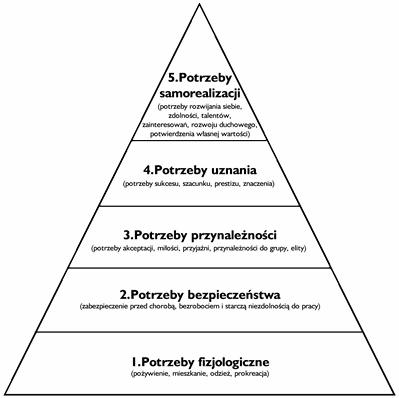
\includegraphics[scale=0.5]{assets/maslow}\\
\end{center}

Potrzeby od dołu piramidy:
\begin{enumerate}
	\item potrzeby fizjologiczne -- pożywienie, mieszkanie, odzież, prokreacja
	\item potrzeby bezpieczeństwa -- zabezpiecznie przed chorobą, bezrobociem i starczą niezdolnością do pracy
	\item potrzeby przynależności -- potrzeby akceptacji, miłości, przyjaźni, przynależności do grupy, elity 
	\item potrzeby uznania -- potrzeby sukcesu, szacunku, prestiżu, znaczenia
	\item potrzeby samorealizacji -- potrzeby rozwijania siebie, zdolności, talentów, zainteresowań, rozwoju duchowego, potwierdzenia własnej wartości
\end{enumerate}

(Instynktywistyczna) teoria potrzeb wg Bronisława Malinowskiego (naukowa teoria kultury)\\

Kultura jako aparat do zaspokajania potrzeb i zespół reakcji na te potrzeby\\
Potrzeby -- Imperatywy kulturowe
\\

\textbf{Szkołą behawioralna -- Teoria XY Douglasa McGregora} (1906 -- 1964)\\

\begin{center}
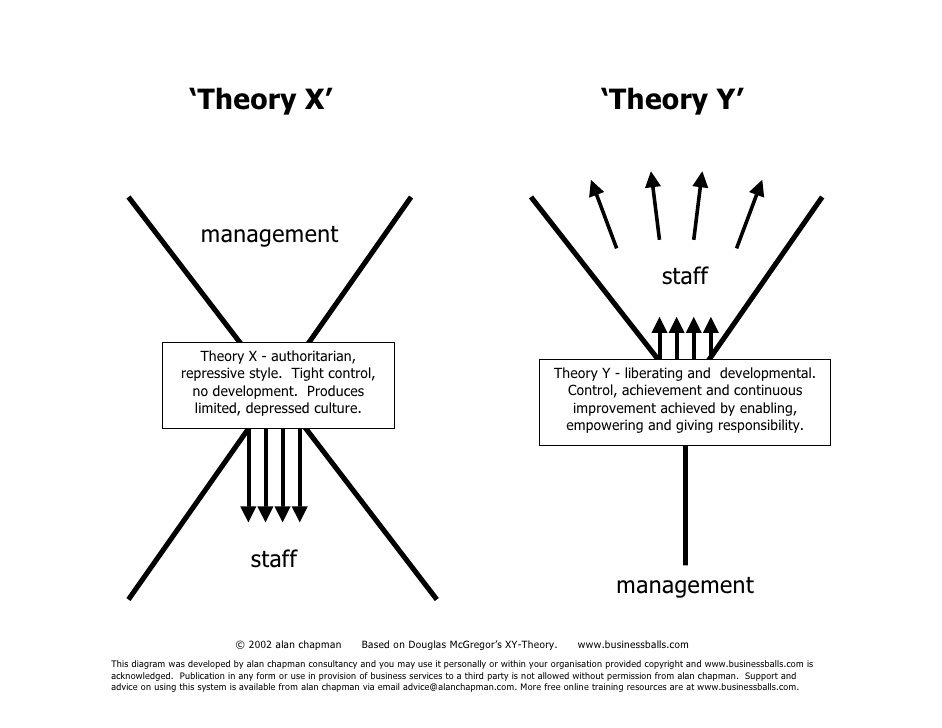
\includegraphics[scale=0.35]{assets/teoriaxy} \\
\end{center}

\begin{itemize}
	\item Teoria Y -- praktyczne zastosowanie "psychologii trzeciej siły" Abrahama Maslowa
	\begin{itemize}
		\item człowiek lubie pracować, chce pracować
	\end{itemize}
\end{itemize}

\noindent\rule{\textwidth}{1.pt}

State od the GLobal Workplace Report 2013 \\
3 kategorie zaangażowania oraz rekomendacje
\begin{itemize}
	\item Engaged -- zaangażowani
	\item Not engaged -- niezaangażowani
	\item Actively disengaged -- wrodzy
\end{itemize}
\begin{center}
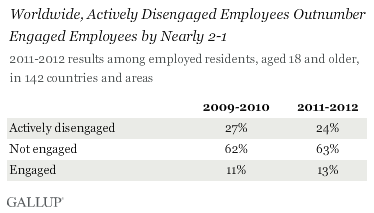
\includegraphics[scale=0.9]{assets/workplacereport}\\
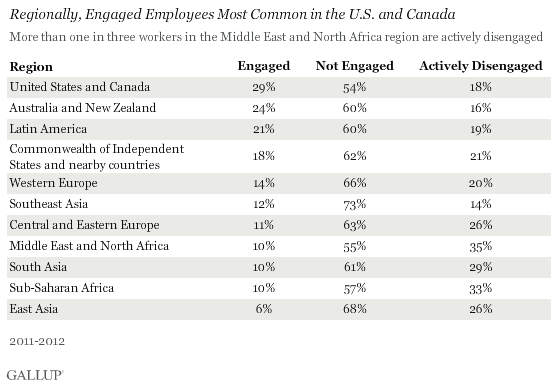
\includegraphics[scale=0.8]{assets/workplacereport2}\\
\end{center}

Polska: [Engaged, Not Engaged, Actively Disengaged] = [17\%, 68\%, 15\%]

\section{31 III 2015 (Górski)}

\textbf{Szkoła ilościowa} \\

Stosowanie metod matematycznych do budowania modeli, analizy i rozwiązywania problemów zarządzania.\\
Inaczej: podejście systemowo-infomatyczne.\\
Przedstawiciele:
\begin{itemize}
	\item P.M. Blackett, J.D. Bernal -- optymalizacja danych
	\item R. McNamara (1916-2009) -- system ilościowego zarządzania w korporacjach
	\begin{itemize}
		\item Polityk i menedżer
		\item z wykształcenia ekonomista i filozof
		\item pierwszy w historii prezes firmy Ford spoza rodziny Fordów (1960 r.)
		\item Sekretarz obrony USA w latach 1961 -- 1968 (za czasów Johna Kennedy'ego)
		\begin{itemize}
			\item Operacja w Zatoce Świć (1961) z udziałem wyszkolonych przez CIA kubańskich uchodźców
			\item Zakończenie kryzysu kubańskiego (10.1962)
		\end{itemize}
		\item Prezes Banku Światowego w latach 1968 -- 1981
		\item Jeden z twórców analizy politycznej (systemowej)
	\end{itemize}
\end{itemize}

Ewolucja nauk o organizacji i zarządzaniu:
\begin{itemize}
	\item poszerzenie perspektywy zainteresowań od stanowiska pracy do złożonych sieci organizacji
	\item przenoszenie zainteresowań z organizacji na otoczenie
	\item ewolucja traktowania organizacji
\end{itemize}

Współczesne koncpecje zarządzania
\begin{itemize}
	\item zarządzanie jako sprawowanie władzy w organizacji
	\item zarządzanie przez delegowanie uprawnień
	\begin{itemize}
		\item zarządzanie na każdym stanowisku pracy
		\item empowerment pracowników
	\end{itemize}
	\item zarządzanie problemami
	\begin{itemize}
		\item identyfikacja i rozwiązywanie problemów
	\end{itemize}
	\item zarządzanie czasem
	\item zarządzanie przez wyjątki
	\item zarządzanie przez cele
	\begin{itemize}
		\item skuteczność -- aby być skutecznym musimy mieć dobrze zformułowane cele
	\end{itemize}
	\item zarządzanie konfliktami
\end{itemize}

4 cechy (paradygmaty) "nowoczesnego zarządzania"
\begin{enumerate}
	\item efektywność (stosunek osiągniętego zysku do poniesionych nakładów)
	\item zdolność elastycznego adaptowania się do zmieniających się warunków (adaptacja do otoczenia)
	\item zdolność systemu do maksymalnego wykorzystania tych aktywów, które wyróżniają dany system spośród innych (przewaga konkurencyjna)
	\item zdolność do generowania celów społecznie akceptowalnych
\end{enumerate}

"Najbardziej istotnym elementem w planowaniu nie jest wskazywanie indywidualnych i ograniczonych celów, lecz świadomość skutków jakie na dłuższą metę cele indywidualne będą miały dla szerszych celów."  
\begin{flushright}
	L. Mannheim
\end{flushright}

\chapter{Temat 4 -- "Strategia poprzedza strukturę" -- Podstawy zarządzania strategicznego}

\section{31 III 2015 (Górski)}

Współcześnie większy nacisk kładzie się na strategię niż strukturę. \\

"Generacja zarządzania" -- czy zarządzanie strategiczne i marketingowe było zawsze obowiązującym paradygmatem?

\begin{itemize}
	\item 1880
	\begin{itemize}
		\item \textbf{zarządzanie przedsiębiorcze}
		\item wyzwanie: jak wzrosnąć w siłę?
		\item paradygmat: wygyrwa silnieszy i bardziej bezwzględny
	\end{itemize}
	\item 1930
	\begin{itemize}
		\item \textbf{zarządzanie funkcjonalne}
		\item wyzwanie: jak zwiększyć skalę działania?
		\item paradygmat: wygrywa wydajnieszy
	\end{itemize}
	\item 1970
	\begin{itemize}
		\item \textbf{zarządzanie marketingowe}
		\item wyzwanie: jak rozszerzyć dominium (rynek)?
		\item paradygmat: wygrywa bardziej konkurencyjny
	\end{itemize}
	\item 1990
	\begin{itemize}
		\item \textbf{zrządzanie strategiczne (marketingowe)}
		\item wyzwanie: jak stawać się bardziej skutecznym i bardziej efektywnym?
		\item paradygmat: wygrywa mądrzejszy i szybszy
	\end{itemize}
\end{itemize}

\textbf{Strategia}\\
"Esencją strategii jest decyzja dotycząca wyboru prowadzenia działań inaczej niż konkurencja po to, aby dostarczyć wyjątkową propozycję wartości." 
\begin{flushright}
	Michael E. Porter
\end{flushright}

Strategia to nie jest dokument, strategią jest decyzja i sposób podejmowania decyzji. Chcemy być inni nie dlatego, aby być innym, tylko żeby dostarczać inne wartości (Unique Selling Point).\\

\textbf{Strategia -- plan biznesu} \\
"Typową reakcją kierownictwa na brak wyraźnie określonego celu jest zwiększenie nakładów: zatrudnienie większej liczby ludzi, zawyżenie kwalifikacji, nacisk na pracowników, by pracowali ciężej"
\begin{flushright}
	Laurence J. Peter
\end{flushright}

Peter dowodzi, że to jest nieskuteczne. Brak strategii jest nieefektywny. Zwiększamy wymagania, nacikamy na wydajność, aby osiągnąć cel -- ale nie wiemy jaki jest ten cel. 

Co to jest strategia?
"Strategoa jest ogólnym programem definiowania i realizacje celów firmy oraz spełnienia jej misji."
\begin{flushright}
	J. Stoner
\end{flushright}

"Strategia wyraża cele długoterminowe przedsiębiorstwa, odpowiadające generalnym kierunkom działania, a także przedstawia alokację zasobów jakie są niezbędne do relaizacji przyjętych cełów"
\begin{flushright}
	A.D.Chandler
\end{flushright}

"Strategia polega na antycypacji zmian otoczenia i dostosowywaniu się do nich. Strategia zawieraa określenie i oszacowanie alternatycwnych sposobów osiągniecią ustalonej misji i celów firmy"
\begin{flushright}
	L.W.Rue
\end{flushright}

\textbf{Strategia jako 5P} -- Henry Mintzberg
\begin{itemize}
	\item strategia jest długofalowym planem (\textbf{plan}) poprzedającym osignięcie świadomie zamierzonych celów
	\item strategia jako manerwr, podstęp (\textbf{ploy}) polegający na przekazywaniu konkruentom sygnałow rynkowych gróźb, że dana firma podejmie jakieś działanie
	\item strategia jest wzrozem (\textbf{pattern}), ziorem różnych działań i decyzji, prowadzącym do spełnienia planów firmy
	\item strategia jest powiązana z określeniem takie pozycji (\textbf{position}) firmy w otoczeniu konkurencyjnym, która gwarantowałaby ookonanie lub unikanie konkurencji (tzw. nisza rynkowa)
	\item strategia jest perspektywą (wizją -- \textbf{perspective}) działania całej firmy identyfikowaną i podzialaną przez wszystkich pracowników.
\end{itemize}

Cel procesu formułowanie strategii to odpowiedzi na pytania:
\begin{itemize}
	\item Jaką pozycję zajmuje obecnie instytucja i jakie są jej możliwości rozwojowe?
	\item Jaką pozycję chcaiłaby zająć w przyszłości i jakie cele chce osiągnąc w okresie strategicznym?
	\item Co jej utrudnia obecnie i co może utrudniąc w przyszłości osiągnięcie zamierzonej pozycji?
	\item Co powinna i co musi uczynić, aby przesunąć się z pozycji zajmowanej na pozycję pożądaną i osiągnąć sukces?
\end{itemize}

Pytania do tworzenie strategii (przykładowe):
\begin{enumerate}
	\item Kim sią moi klienci?
	\item Jak się zmieniają priorytet klientów?	
	\item Kto powinien być moim klientem?
	\item W jaki sposób mogę zwiększyć wartośc dla klienta?
	\item W jaki sposób mogę doprowadzić do tego, żeby klient przede wszystkim wybierał mnie?
	\item Jaki jest mój model zysku?
	\item Jaki jest mój obecny model działalności firmy?
	\item Kim są moi prawdziwi konkurenci?
	\item Jakie są modele działalności moich najgroźniejszych konkurentów?
	\item Jaki będzie mój najlepszy model działalności firmy?
	\item Jaki jest mój punkt punkt kontroli strategicznej? (KPI -- Key Performance Indicators)
	\item Ile jest warta moja firma?
\end{enumerate}

4 główne skłądowe strategii
\begin{enumerate}
	\item \textbf{Domena działania}
	\begin{itemize}
		\item gdzie i komu organizacja zamierza sprzedawać swoje wyroby/usługi?
	\end{itemize} 
	\item \textbf{Strategiczna przewaga}
	\begin{itemize}
		\item w ramach danej domeny w stosunku do konkurentów
	\end{itemize}
	\item \textbf{Cele do osiągnięcia}
	\begin{itemize}
		\item cele strategiczne -- co chcemy osiągnąc w kolejnych okresach?
		\item jak długie okresy rozważamy? Głównie się decyduje na okresy 3-5 lat... ale to zależy od branży.
	\end{itemize}
	\item \textbf{Funkcjonalne programy działania}
	\begin{itemize}
		\item przełożenie strategii na konkretne działania w obszerach funkcjonalnych
	\end{itemize}
\end{enumerate}

\textbf{Podejścia do strategii}
\begin{itemize}
	\item Stare:
	\begin{itemize}
		\item .
	\end{itemize}
	\item Nowe:
	\begin{itemize}
		\item .
	\end{itemize}
\end{itemize}

\section{9 IV 2015 (Opolski)}

Nowa fala w zarządzaniu\\

Peters i Waterman sformułowali \textbf{8 cech "idealnego przedsiębiorstwa"}
\begin{itemize}
	\item obsesja działania
	\item bliski i bezpośrdeni kontakt z klientem
	\item autonomia i przedsiębiorczość (pracowników)
	\item wydajność i efektywność (kadry najważniejszym systemem)
	\item koncentracja na wartościach (specyficzny system działania)
	\item wykorzystywanie kluczowych kompetencji
	\item prosta struktura, niewielki sztab (odchudzenie kierownictwo)
	\item symbioza luźnych i sztywnych form w 1 strukturze
\end{itemize}

\textbf{Tradycyjne a nowe podejście do strategii}

\begin{itemize}
	\item Model tradycyjney
	\begin{itemize}
		\item Reaktywne
		\begin{itemize}
			\item doraźne
			\item interwencje cząstowe -- gdy powstaje "problem"
		\end{itemize}
		\item Kadry jako pozycja po stronie wydatków "koszty zmienne"
		\item Dominują orientacje na własne "egoistyczne" interesy
		\item pracownicy starają się poszerzuć zakres własnych wpływów w drodze do przetargów i konfrontacji
		\item kontrola przepływu informacji mająca na celualbo wzrost wydajności, albo poszerzenie wpływów
		\item orientacja na "stosunki międzyludzkie"
		\item kontrola odgórna
	\end{itemize}
	\item Model nowoczesny (strategiczny)
	\begin{itemize}
		\item proaktywne systematyczne działanie mające na celu harmonizację:
		\begin{itemize}
			\item HRM i planowania strategicznego organizacji
			\item zmian kultury organizacyjnej
			\item przydziału stanowisk, awansów, zwolnień itp. z wymogami wzorów nowoczesnej kultury organizacyjnej
			\item zmian organizacyjnych
		\end{itemize}
		\item Kadry jako kapitał społeczny, który powinien być rozwijany poprzez:
		
		\begin{itemize}
			\item rozwój nowoczesnych form pracy zawodowej
			\item zachęcanie pracowników do poszerzania kompetencji zawodowych i wdrażanie systemów płacowych motywyujących do tego
			\item kompleksowe wykorzystanie szkoleń
			\item swobodne komunikowanie się w organizacji i współudział pracowników w zarządzaniu
			\item nacisk na bezpieczeństwo zatrudnienia
			\item nacisk na rowzwój kapitału społecznego
			\begin{itemize}
				\item Kapitał ludzki -- to moja wiedza, a kapitał społeczny to coś więcej. Polega na kooperacji między jednostkami.
			\end{itemize}
		\end{itemize}
		\item Dominują interesy kooperacyjne
		\begin{itemize}
			\item wspólny wysiłek kierownictwa i pracowników mający na celu jakość środowiska pracy i wydajność pracy
			\item nacisk na poczucie własnej wartości pracowników, które owocuje pozytywnymi rezultatami z punktu widzenia firmy i psychoologiczną sytuację pracownika
		\end{itemize}
		\item nacisk na złagodzenie nierówności podziału władzy w organizacji, a przez to rozwój zaufania i współpracy
		\begin{itemize}
			\item ścisła wspołpraca ze związkami zawodowymi; uczestnictwo związku w podejmowaniu istotnych decyzji
			\item odejście od symboliki podkreślającej różnice statusu
		\end{itemize}
		\item Swobodny przepływ informacji w celu budowy zaufania i współdecydowania pracowników
		\begin{itemize}
			\item upowszechnienie informacji na temat firmy i jej planów
			\item upowszechnienie informacji na temat celów i założeń systemów płacowych
		\end{itemize}
		\item orientacja przede wszystkim na cele organizacji
		\begin{itemize}
			\item cele produkcyjne powinny być jasne i zrozumiałe
			\item pracownicy powinni w pewnym zakresie uczestniczyć w formułowaniu celów organizacji
		\end{itemize}
		\item współuczestnictwo i możłiwość świadomego wybory
		\begin{itemize}
			\item partycypacyjn styl zarządzania
			\item programy mające na celu wzrost zainteresowania i zaangażowania pracowniów w sprawy firmy
			\item wpływ pracowników na przebieg ich orgranizacyjnych karier
			\item elastyczne struktury organizacyjne; zespoły zadaniowe
		\end{itemize}
	\end{itemize}
\end{itemize}

zasady zarządzania strategicznego

\begin{enumerate}
	\item Zasada celowości (Misja, Wizja, Cel)
	\item Zasady myślenia strategicznego -- Stosowania kompleksowej analizy sytuacji zewnętrznych w wewnętrznych uwarunkowań działań instytucji (SWOT)
	\begin{itemize}
		\item przedkładanie celów perspektywicznych nad celami bieżacymi
		\item szybkie przekształcenie struktur, procedur i zadań odpowiednio do sytuacji wewnętrznych i wymogów działania
		\item elastyczność działania
	\end{itemize}
	\item zasada zachowania strategicznego
	\begin{itemize}
		\item antycypacja w przygotowaniu instytucji do zmian w otoczeniu oraz kształtowanie warunków sprzyjających wrzechstronnemu rozwojomi instytcji
\end{itemize}
	\item zasada podejścia sytemowego
	\begin{itemize}
		\item dązenie do osągnięcia i utrzymania spójności wszystkich składowych danej całości ze względu na założone cele
	\end{itemize}
	\item zasada przewagi konkurencyjnej
	\begin{itemize}
		\item umiem coś robić lepiej niż konkurencja
		\item przewaga konkurencyjna jest względnie trwała (nieprzypadkowo)
		\item musi być zakomunikowana; klient musi o tym wiedzieć
	\end{itemize}
	\item zasada kreatywności
	\item zasada rozwijania wiedzy ludzkiej
	\item zasada wykorzystywania kluczowych kompetencji
	\item zasada integracji z firmą
\end{enumerate}

Proces tworzenia organizacji. 
\begin{center}
	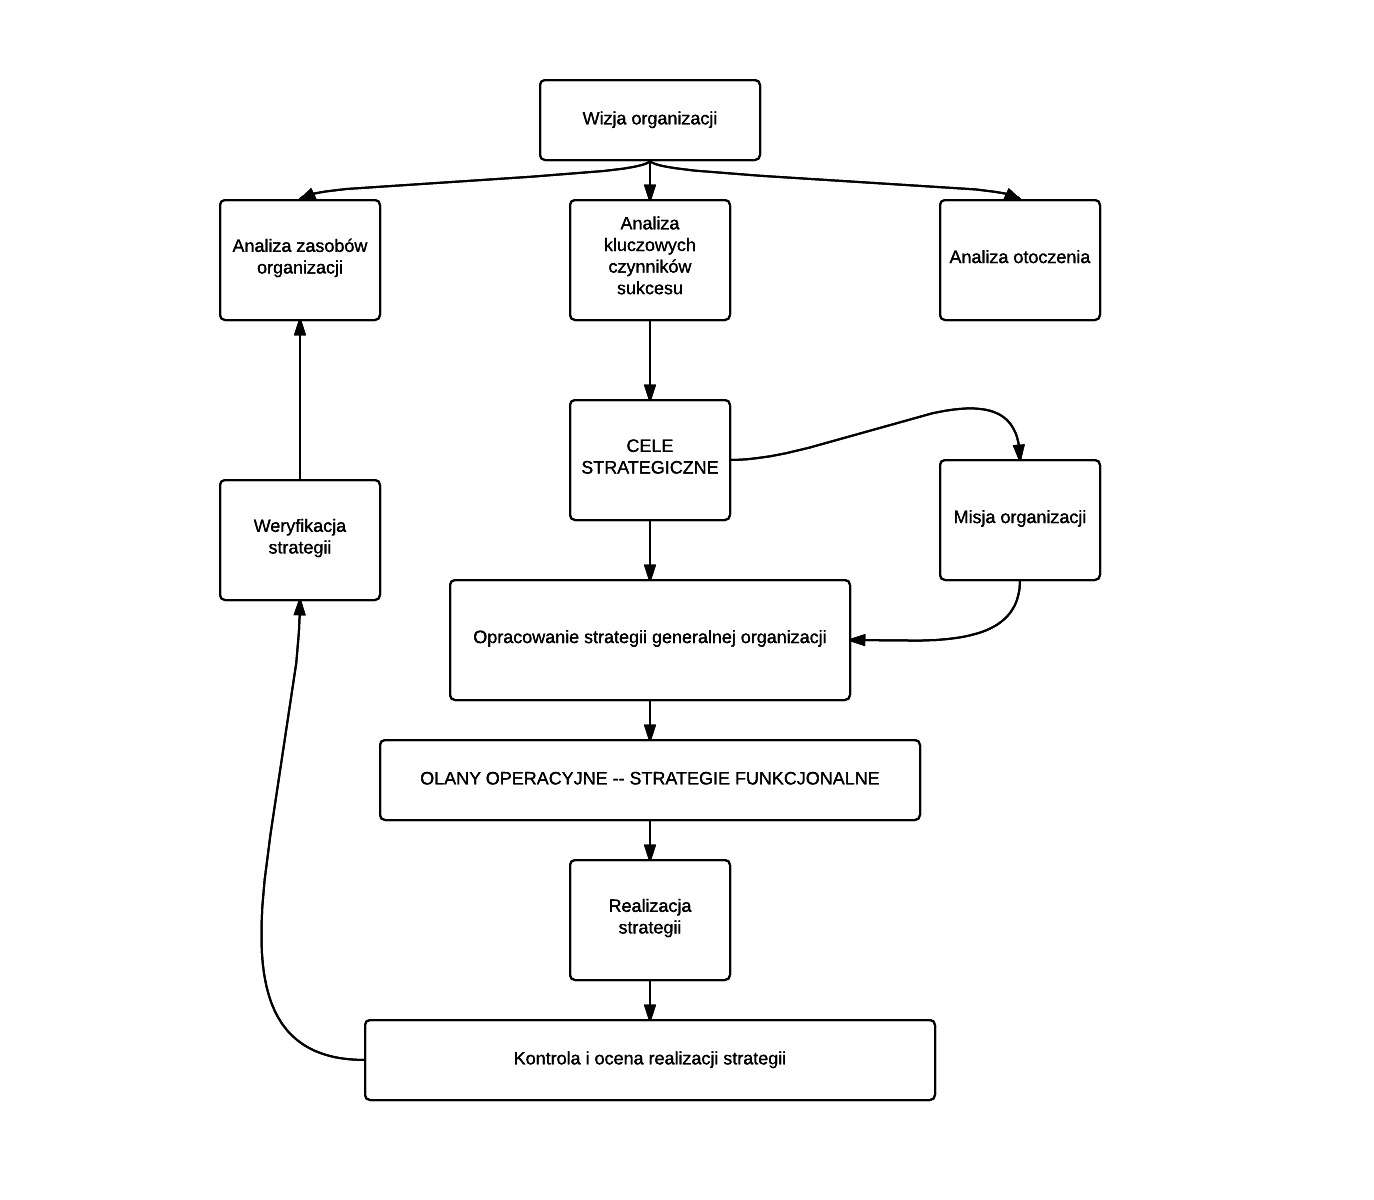
\includegraphics[scale=0.7]{assets/procestworzeniastrategii.png}
\end{center}

Strategie głównie buduje się głównie na okres 3 lat. Prognoza, projekcja jest na dłuższy okres (np. Polska 2040).
\\
Trochę absurdalna była misja Brytyjskich Kolei Żelaznych: "Dowieziemy Cię tam, gdzie zechcesz."
\\
Misja nie może być fałszywa (w USA pojawiają się pozwy pracownicze przeciwko firmą, ze względu na to).

\section{14 IV 2015 (Górski)}

\textbf{Analiza SWOT} -- narzędzie diagnostyczne
\begin{itemize}
	\item SWOT -- metodologia analizy strategicznej organizacji
	\begin{itemize}
		\item S -- strengths -- mocne strony organizacji
		\item W -- weaknesses -- słae strony organizacji
		\item O -- opportunities -- szanse w otoczeniu
		\item T -- threats -- zagrożenia w otoczeniu
	\end{itemize}
	\item Pełni głównie funkcje diagnostyczne, ale jest także narzędziem ukierunkowującym usprawnienie organizacji i jej funkcjonowania
\end{itemize}

SWOT jest pomiędzy aktualną sytuacją, a przyszłą sytuacją.
\begin{itemize}
	\item Aktualna sytuacja
	\begin{itemize}
		\item Co jest przedmiotem naszej oferty?
		\item Kto wspomaga naszą działalność?
		\item Kim są nasi nabywcy?
		\item Kto jest ważny dla organizacji
		\item Czym dysponujemy obecnie w procesie świadczenia usług?
	\end{itemize}
	\item przyszła sytuacja
	\begin{itemize}
		\item Kim będziemy?
		\item Komu będziemy oferować usługi?
		\item Jak będziemy świadczyć usługi?
		\item Jaki zespół pracowników będziemy mieć?
		\item Jakimi zasobami materialnymi i fifnansowymi będziemy dysponować?
		\item Kto poprze nas autorytetem finansowo lub pracą?
	\end{itemize}
\end{itemize}

SWOT nei jest narzędziem do inwentaryzacji.

\begin{center}
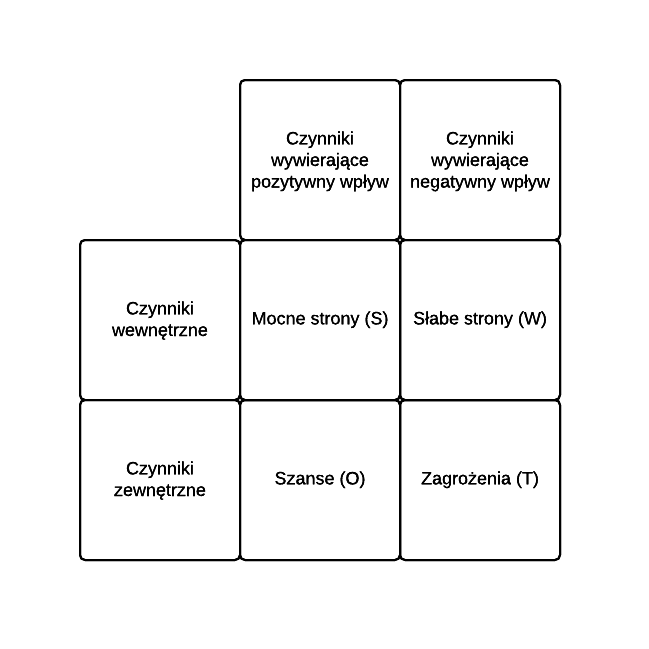
\includegraphics[scale=0.87]{assets/SWOT}
\end{center}

SWOT -- racjonalny wybór okazji \\

"Ważną rzeczą w życiu jest wiedzieć, kiedy skorzystać z okazji, ale nie mniej ważne jest wiedzieć, kiedy nie należy z niej skorzystać"
\begin{flushright}
Benjamin Disraeli
\end{flushright}

\begin{center}
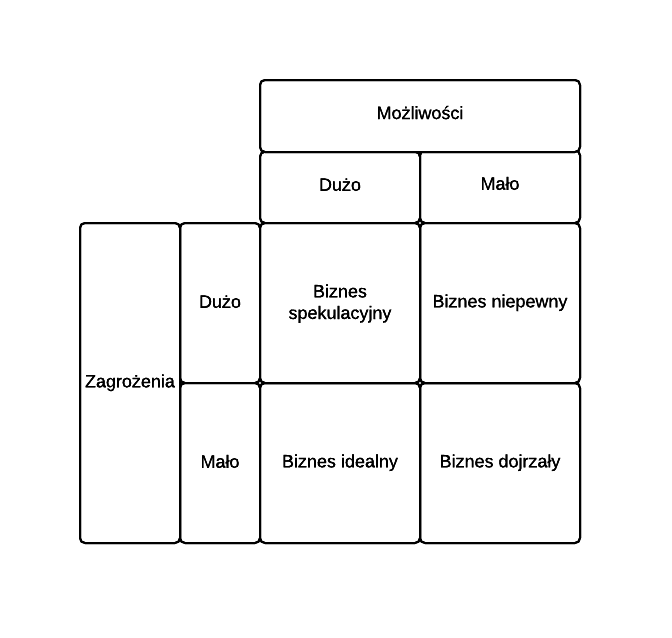
\includegraphics[scale=0.87]{assets/SWOT2}
\end{center}

Argumenty w analizie SWOT muszą być ważne dla firmy. Musi być przyczynowość i adekwatność.
\\

Punktowe oszacowanie czynników SWOT -- przykład mocnych stron \\
\begin{tabular}{| c | c | c| c | c |}
\hline
L.P. & Mocna Strona (S) & Waga (\%) & Ocena (Od 1 do 5) & Ocena ważona \\ \hline
1 & Unikalna technologia wytwarzania polimerów & 20\% & 5 & 1 \\ \hline
2 & Zaawansowany system dystrybucji elektronicznej & 15\% & 3 & 0.45 \\ \hline
3 & Niskokosztowe kanały promocji sprzedaży & 10\% & 5 & 0.4 \\ \hline
(...) & - & - & - & \\ \hline

\end{tabular}

SWOT -- Jak wybrać kierunek strategiczny\\
Kiedy obliczymy sumaryczną ilość punktów dla każdej z czterech grup czynników (S, W, O, T), można określić

\begin{itemize}
	\item Atrakcyjność rynkowa (AR) AR = O/(O+T)
	\item Pozycję rynkową (PR) PR = S/(S+W)
	\item Prawdopodobieństwo Sukcesu Strategicznego (PSS)PSS = 1/2(AR + PR)
	\item Wartość graniczna dla sukcesu strategicznego: 0.5
\end{itemize}

\begin{center}
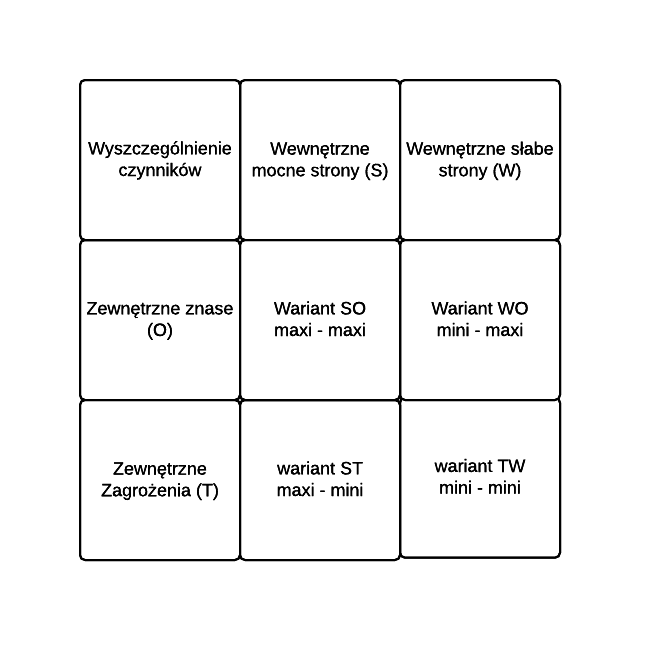
\includegraphics[scale=1]{assets/SWOT3}
\end{center}

\textbf{Macierz Ansoffa}
\begin{itemize}
	\item Macierz Ansoffa to narzędzie służące dokonywaniu wyborów startegicznych co do dalszej ścieżki rozwoju, w zakresie strategii rynku oraz strategii oraz strategii produktu
	\item Najczęsciej po to narzędzie siega się na etapie dojrzałości produktu w jego cyklu życia, gdy poszukuje się metod zwiększania sprzedaży i zysku firmy
	\item Macierz daje 4 możliwości strategiczne, przy czym:
	\begin{itemize}
		\item Najpierw ocenia się szanse penetracji rynku
		\item Następnie ocenia się możliwość zaistnienie z dotychczasową (...) 
		\item (...no time...)
	\end{itemize}
\end{itemize}

Macierz ansoffa -- \textbf{strategie rozwoju}
\begin{center}
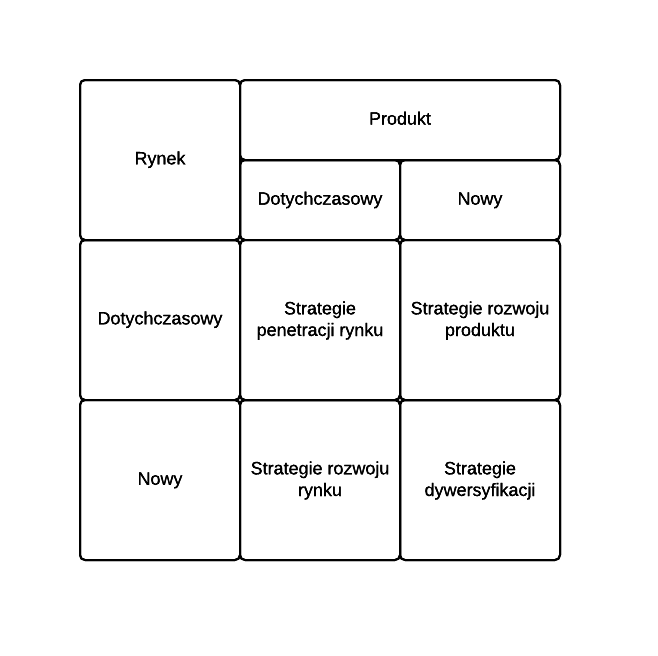
\includegraphics[scale=0.82]{assets/Ansoff}
\end{center}

\textbf{Strategie ograniczania}
\begin{center}
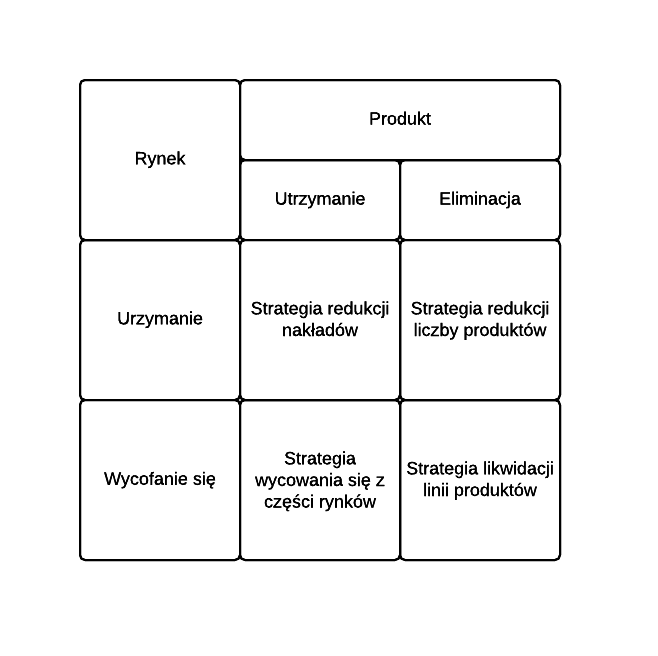
\includegraphics[scale=0.82]{assets/Ansoff2}
\end{center}

\textbf{Powrót do korzeni -- misja i wizja} \\

"Misja firmy to jej rola, sens istnienia. WIzja - to koncepcja jej potencjału, wyobrażenie pożadanej przyszłości"
\begin{flushright}
Richard Koch
\end{flushright}

Funkcję dobrej misji:
\begin{itemize}
	\item misja jako punkt określenia -- funkcja ukierunkowująca
	\item misja jako deklaracja intencji -- funkcja uwiarygadniająca
	\item misja jako wartość -- funkcja integrująca
	\item misja jako gwarancja przyszłości -- funkcja stabilizująca
	\item misja jako źródło natchnienia -- funkcja inspirująca
\end{itemize}

\textbf{Misja firmy -- deklaracja strategiczna}\\
Misja firmy powinna być deklaracją wynikającą z długofalowej strategii w co najmniej z pięcu obszarów:
\begin{enumerate}
	 \item Domena -- profil działalności albo portfel strategicznych bilansóœ firmy
	 \item Odpowiedzialność -- stosunek firmy do ważnych partnerów
	 \item Sukces -- standardy - kryteria wg których mierzyć będziemy powodzenie firmy
	 \item Kompetencje -- kluczowe zdolności i umiejętności wspomagające osiągnanie sukces
	 \item Organizacja -- zestaw głównych reguł wg których skonstruowany jest system zarządzania firmą
\end{enumerate}

\textbf{Przykłady misji:}
\begin{enumerate}
	\item Texaco
	\begin{itemize}
		\item Być jedną z najbardziej uznanych, zyskownych i konkurencyjnych i uczynić Texaco liderem w branży
		\item misja typu: "król jest tylko jeden" 
	\end{itemize}
	\item Internal Revenue Service
	\begin{itemize}
		\item Obiecujemy należycie i najniższym kosztem zabezpieczać wszystkie powierzone nam deklaracje podatkowe
		\item jest to przykład dobrej misji
	\end{itemize}
\end{enumerate}

Misja firmy a zamiar strategiczny
\begin{itemize}
	\item Zamiar strategiczny -- ogólny średnio- lub długoterminowy strategiczny cel firmy
	\begin{itemize}
		\item Ford: "zdemokratyzować samochód"
		\item Honda: "rozgromić Yamahę"
	\end{itemize}
	\item idelana sytuacja strategiczna 00 wygenerowanie "wznoszącej się spirali (\textbf{virtous circle} -- przeciwieństwo vicouis circle)
\end{itemize}

\textbf{Virtous circle w strategii}
\begin{center}
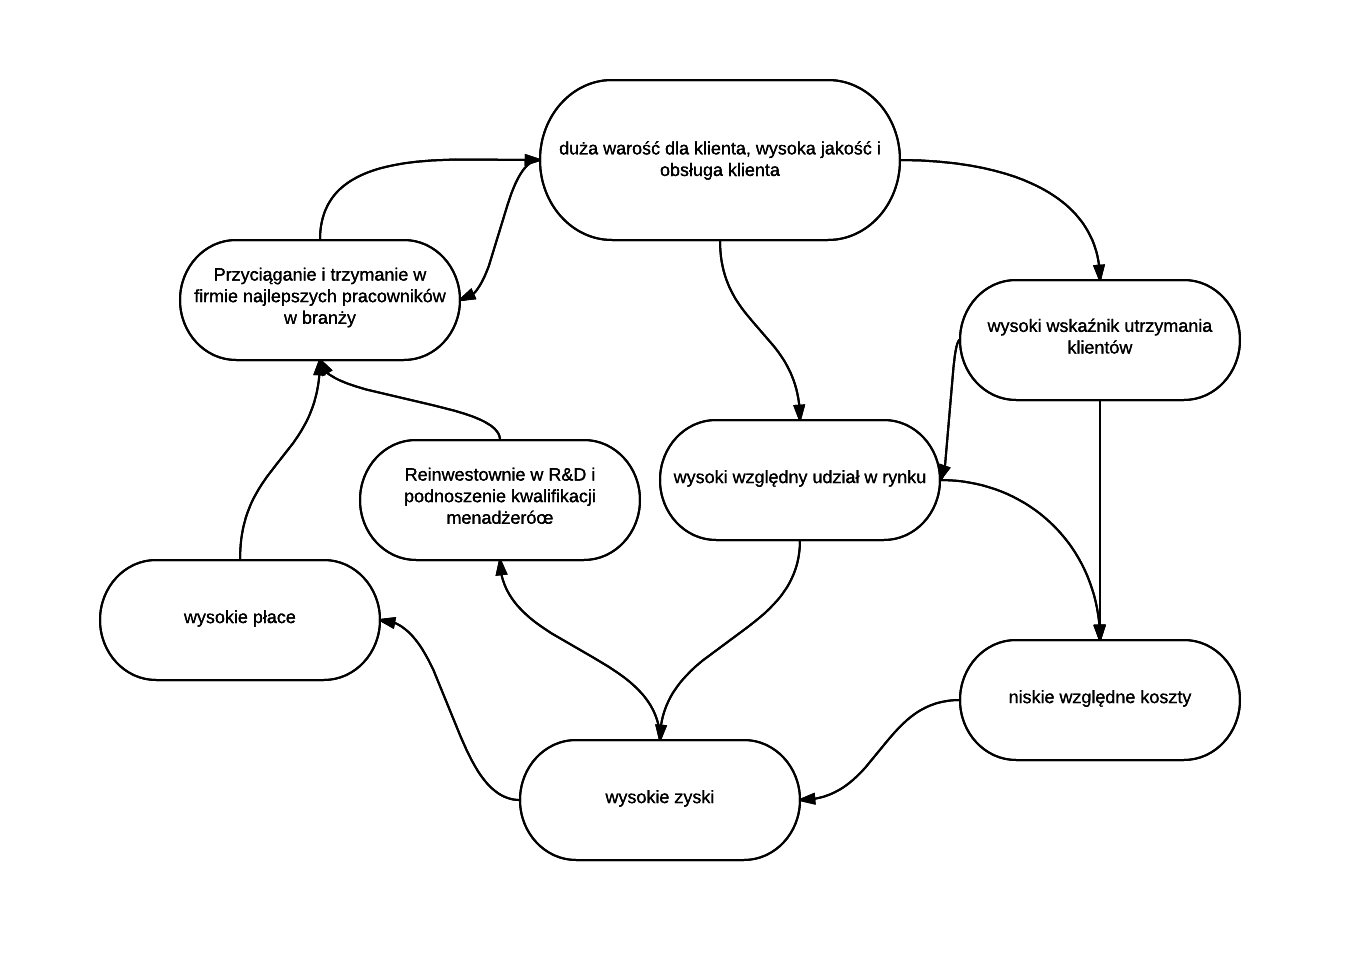
\includegraphics[scale=0.7]{assets/circle}
\end{center}

Misja firmy a wartości wg Jack'a Welcha (CEO GE 1981 -- 2001)
\begin{itemize}
	\item Podczas gdy misja firmy mówi o tym, dokąd zmierzacie, wartości firmy opisują zachowanie, które pozwoli wam dojść do celu
	\item Menedżerowie często pomijają tę część planowania drogi do zwycięstwa, choć ich podwładni powinni te wartości traktować jak rozkazy bojowe
	\item wartości to sposób działania w czasie misji, droga do celu, czyli zwycięstwa
	\item Rozwijanie wartośc, które będą wspierać waszą misję, wymaga zaangażowania całej załogi i kadry kierowniczej. Te cztery wskazówki pozwolą wam zaplanować ten proces
\end{itemize}

Budowanie misji i wartości. 4 wskazówki Jack'a Welcha
\begin{enumerate}
	\item Proces tworzenia wartości musi się składać z ciągłych powtórzeń i doskonalenia
	\item Opis musi być konkretny
	\item Aby wartości rzeczywiście coś znaczyły firma musi nagradzać pracownikwów, którzy się do nich stosują i "karać" tych, którzy tego nie robią
	\item aby misja firmy i jej wartości współgrały ze sobą i pozwoliły zwyciężać, muszą się wzajemnie uzupełniać
\end{enumerate}

Przewaga konkurencyjna jako podstawa strategii
\begin{itemize}
	\item Odpowiadamy na pytania
	\begin{itemize}
		\item co takiego posiadamy czego nie ma konkurencja
		\item czym chcemy wygrać z konkurentami, co będzie źródłęn naszej rynkowej przewagi?
	\end{itemize}
	\item Podkreślamy zalete, ale nie ukrywajmy słabszych stron strategii (realistyczna ocena ryzyka)
	\item Najczęściej misja firmy i jej wartości przepadają na skutek kryzysóœ dnia codziennego [Jack Welch]
\end{itemize}

\textbf{Skuteczne strategie przewagi konkurencyjnej}1\\
Na podstawie badań firm stosujących BSC (Treacy, Wiersema) zauważono, że są 3 strategie przewagi konkurencyjnej
\begin{enumerate}
	\item \textbf{Przywództwo produktu} (np. Sony, Intel)
	\begin{itemize}
		\item Promowanie innowacyjności
		\item Styl zarządzania zorientowany na ryzyko
		\item Uznanie, że źródłem sukcesu są ludzie obdarzeni nieprzeciętnymi zdolnościami
		\item Uznanie konieczności praowdzenia edukacji rynkowej w zakresie korzyści z innowacji produktowych
	\end{itemize}
	\item \textbf{Zażyłość z klientem} (np. Home Depot Inc, Mobil)
	\begin{itemize}
		\item Posiadanie pełnego asortymentu usług/produktów dostępnych na żadanie klienta
		\item Filozofia zarządzania zorientowana na pełne zrozumienie oczekiwań klientóœ (consumer insight)
	\end{itemize}
	\item \textbf{Doskonałość operacyjna}: kombinacja jakości, ceny i łatwości transakcji (no. McDonald's, Dell)
	\begin{itemize}
		\item Skuteczne i efektywne zarządzanie personelem
		\item Koncentracja na efektywności operacji biznesowych
		\item Dbałość o systemy pomiaru
		\item Zarządzanie oczekiwaniami klientów
	\end{itemize}
\end{enumerate}

\section{16 IV 2015 (Opolski) TODO}

\chapter{Struktury organizacyjne}
\section{21 IV 2015 (Górski)}

\begin{itemize}
	\item Liniowa
	\begin{itemize}
		\item 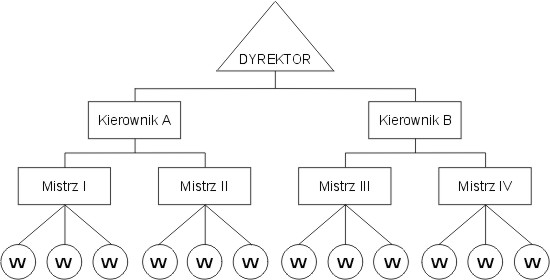
\includegraphics[scale=2]{assets/str_liniowa}
		\item Do każdego pracownika jest jedna ścieżka
		\item Zalety
		\begin{itemize}
			\item duża przejrzystość
			\item jedność rozkazodawstwa
			\item rozłączny podział kompetencji i odpowiedzialności
			\item obowiązywanie drogi służbowej
		\end{itemize}
		\item Wady
		\begin{itemize}
			\item przerwanie drogi służbowej
			\item wydłużenie się kanałów informacyjnych
			\item wzrost formalizacji
			\item brak kompetencji kierowników
			\item mała zdolność przystosowawcza
		\end{itemize}
	\end{itemize}
	\item funkcjonalna
	\begin{itemize}
		\item 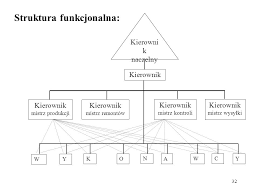
\includegraphics[scale=1.2]{assets/str_funkcjonalna}
		\item Zalety
		\begin{itemize}
			\item specjalizacja stanowisk kierowniczych
			\item łatwe reagowanie na zmiany zewnętrzne
		\end{itemize}
		\item Wady
		\begin{itemize}
			\item srzeczność poleceń wydawanych przez kierowników
			\item trudność w ścisłym rozgraniczeniu kompetencji
			\item dalszy proces specjalizacji kierowników i tworzenie się nowych stanowisk
		\end{itemize}
	\end{itemize}
	\item sztabowo-liniowa
	\begin{itemize}
		\item 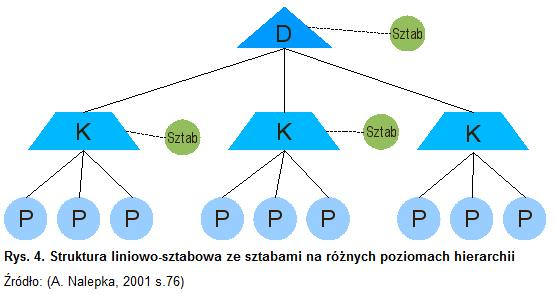
\includegraphics[scale=0.8]{assets/str_sztabowo_liniowa}
		\item sztaby nie są ograniczone strukturą liniową
		\item Zalety
		\begin{itemize}
			\item zasada jedności rozkazodawstwa
			\item zwiękzenie tempa przekazywania poleceń oraz wzbogacenie ich w treść
			\item zalety struktury liniowej
		\end{itemize}
		\item Wady
		\begin{itemize}
			\item przekształcenie w strukturę funkcjonalną (w przypadku, gdy sztaby mają zbyt dużą autonomię)
		\end{itemize}
		\item Parkinson o "komitetach"
		\begin{itemize}
			\item Cykl życia komitetu jest dla naszej wiedzy o sprawach współczesnych czymś tak ważnym, że aż dziwne, iż nie poświęcono więcej uwagi nauce o komitetologii. Pierwsza i najbardziej podstawowa zasada tej nauki to ta, że komitet jest w swej istocie czymś raczej organicznym niż mechanicznym: nie jest on budowlą, lecz rośliną. Zapuszcza korzenie i rośnie, kwitnie, przekwita i więdnie, rozrzucając ziarno, z którego kolejno wykiełkują inne komitety. 
		\end{itemize}
		\item Parkinsonowska "komitetologia"
		\begin{itemize}
			\item \url{http://ms-net.info/teksty,6,3}
		\end{itemize}
	\end{itemize}
	\item pozioma
	\begin{itemize}
		\item Zalety
		\begin{itemize}
			\item umacnia zasadę jedności rozkazodawstwa
			\item wyklucza niebezpieczeństwo samoczynnego przekształcenie się struktury zarządu czy ruchu w strukturę typu funkcjonalnego
		\end{itemize}
		\item Wady
		\begin{itemize}
			\item silne tendencje do przerostu administracji
			\item słabo reaguje na bodźce z otoczenia
			\item skłonność do autonomizacji obu jej części składowych
		\end{itemize}
	\end{itemize}
	\item pionowa
	\begin{itemize}
		\item 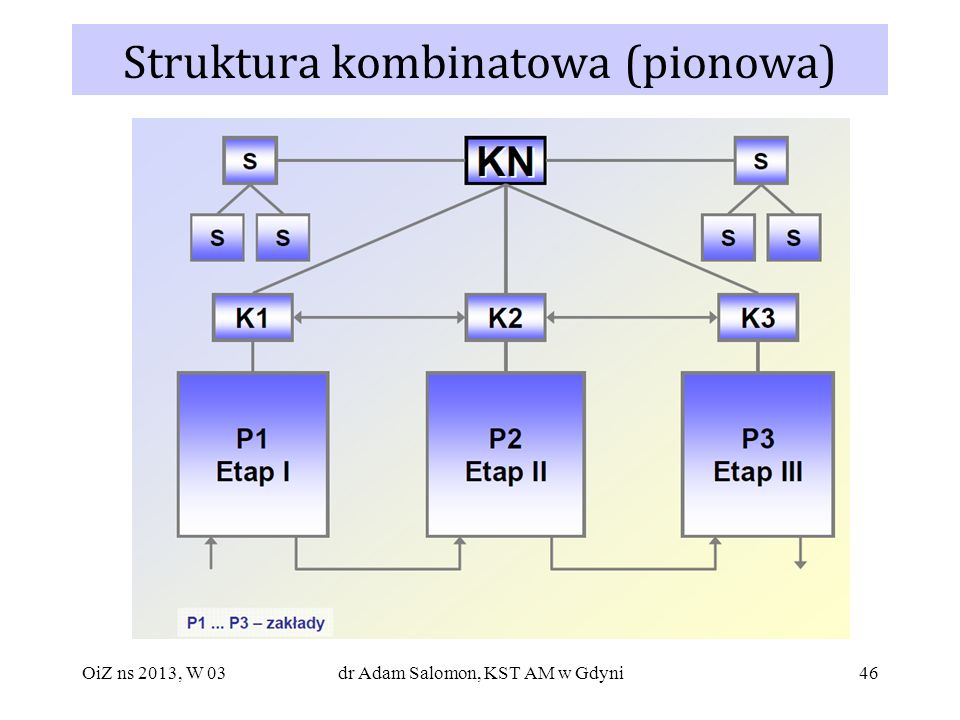
\includegraphics[scale=0.42]{assets/str_pio}
		\item Zalety
		\begin{itemize}
			\item wewnętrzna spójność systemu kierowania
			\item rozgraniczenie rodzajów kierowania: bieżącego i perspektywicznego
		\end{itemize}
		\item Wady
		\begin{itemize}
			\item brak elastyczności
		\end{itemize}
	\end{itemize}	
	\item macierzowa
	\begin{itemize}
		\item 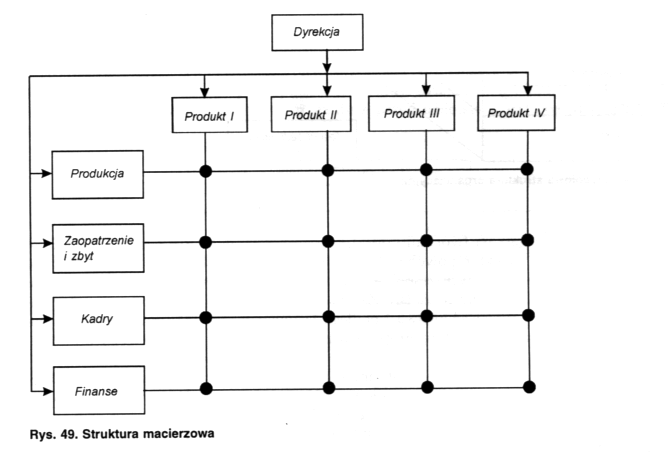
\includegraphics[scale=0.4]{assets/str_macierzowa}
		\item Zalety
		\begin{itemize}
			\item zwiększenie odpowiedzialności za projekt
			\item rozwiązanie wielu problemów organizacyjnych
			\item wyzwolenie inwencji twórczej
			\item lepsze wykorzystanie wiedzy specjalistycznej pracowników
			\item elastyczność
		\end{itemize}
		\item Wady
		\begin{itemize}
			\item powstanie konfliktów kompetencyjnych
			\item wysokie wymagania stawiane kierownikom i podwładnym
		\end{itemize}
	\end{itemize}	
	\item dywizjonalna
	\begin{itemize}
		\item Zalety
		\begin{itemize}
			\item .
		\end{itemize}
		\item Wady
		\begin{itemize}
			\item .
		\end{itemize}
	\end{itemize}
\end{itemize}

Struktury kapitałowe
\begin{itemize}
	\item Struktury kapitałowe działalności gospodarczej to struktury, których elemetem są samodzielne prawne podmioty gospodarcze w postaci spółek kapitałowych
	\item relacje podporządkowania mają charakter kapitałowy
	\item podmiot nadrzędny posiadający udziały lub akcje innych podmiotów określany jest jako spółka dominująca, przedsiębiorstwo macierzyste lub spółka matka
	\item podmioty podrzędne określane są jako spółki-córki
\end{itemize}

Spółki kapitałowe
\begin{itemize}
	\item spółki zależne
	\begin{itemize}
		\item są to podmioty wchodzące w skład strukutr kapitałowych działaności gospodarczej, w których podmiot nadrzędny posiada większość całkowitej liczby głosów w ogranach tych spółek
	\end{itemize}
	\item spółki stowarzyszone
	\begin{itemize}
		\item są to podmioty wchodzące w skład struktur kapitałowych działaności gospodarczej, w któ©ych podmiot nadrzędny posiada 20 - 50\% liczby głosów na zgromadzeniach wspólników lub walnych zgromadzeniach akcjonariuszy
	\end{itemize}
	\item spółki związane
	\begin{itemize}
		\item są to podmioty wchodzące w skład struktur kapitałowych działalności gospodarczej, w któych podmiot nadrzędny posiada mniej niz 20\% liczby głosów
	\end{itemize}
\end{itemize}

Rodzaje grup kapitałowych
\begin{itemize}
	\item holdingi operacyjne
	\begin{itemize}
		\item są to kapitałowe struktury działalności gospodarczej składające się z powiażanych ze sobą kapitałowo lecz samodzielnych prawnie podmiotów gospodarczych w których:
		\begin{itemize}
			\item spółka matak prowadzi operacyjną działalnośc gospodarczą kluczową dla holdingu, a poza tym oddziaływuję właścicielsko na spółki-córki w celu realizacji założoyc hcelów
			\item wpółk-córki prowadzą działalność operacyjną wspierającą działalność operacyjną spółki-matki.
		\end{itemize}
	\end{itemize}
	\item holdingi zarządcze określane również jako strategiczne
	\begin{itemize}
		\item spółka matka nie prowadzi peracyjnej działalności gospodarczej lecz zajmuje się wyłącznie oddziaływaniem właścicielskim na spółki-córki w celu realizacji założoych celów
		\item spółki-córki prowadzą komplementarną działalność operacyjną
		\item wykorzystanie efektów synergicznych
	\end{itemize}
	\item holdingi finansowe
	\begin{itemize}
		\item spółka matka nie prowadzi operacyjnej działalności gospodarczej lecz zajmuje się wyłącznie oddziaływaniem właścicielskim na spółki-córki za pomocą instrumentów finansowych w celu realizacji założonych celów
		\item spółki-córki prowadzą niepowiązaną ze sobą zdywersyfikowaną działalność operacyjną
		\item efekt: maksymalizacja korzyści inwestycyjnych i ograniczenie ryzyka inwestycyjnego spółki matki
	\end{itemize}
\end{itemize}

\chapter{Temat 6: Od problemu do decyzji -- procesy decyzyjne w organizacji}

\section{23 IV 2015 (Opolski)}

\noindent Problem decyzyjny
\begin{itemize}
	\item Jest to odchylenie stanu istniejącego od stanu pożadanego
	\item Rozwiązanie problemu decyzyjnego polega na odpowiedzeniu na pytanie
	\begin{itemize}
		\item jak należy postąpić, by zniwelować różnicę między stanem istniejącym, a stanem pożądanym
	\end{itemize}
\end{itemize}

Podejmowanie decyzji\\
\textbf{Jest to akt świadomego wyboru jednego z rozpoznanych i dostępnych wariantów czegoś co jest przedmiotem wyboru}
\\
\noindent Rozpoznanie wariantów
\begin{itemize}
	\item Należy przewidzieć skutki realizacji każdego z nich
	\item Należy określić prawdopodobieństwo zaistnienia tych skutków
	\item Należy przewidzieć stopień pożadania tych skutków
\end{itemize}

\noindent Diagnoza alternatyw a decyzja
\begin{itemize}
	\item "Z dwojga złego nie wybieraj żadnego" C. Spurgeon
	\item "Jeśli nie wiesz, dokąd idziesz, zajdziesz gdzie indziej" Laurence J. Peter
\end{itemize}

\noindent Fayz podejmowania decyzji
\begin{enumerate}
	\item Definiowanie problemu
	\begin{itemize}
		\item analiza rzeczywistych przyczyn zaistniałych problemów
		\item określenie warunków rozwiązanie problemów
	\end{itemize}
	\item Analiza problemu
	\begin{itemize}
		\item ustalenie celów i reguł postępowania
		\item klasyfikacja problemów
		\item ustalenie faktów
	\end{itemize}
	\item Opracowanie wariantów rozwiązania problemu
	\begin{itemize}
		\item ustalenie listy wariantów
		\item ocena poszczególnych wariantów
	\end{itemize}
	\item wybór najlepszego wariantu
	\begin{itemize}
		\item sformułowanie kryteriów wyboru (ryzyko, dospodarność w wysiłkach, rozkład w czasie)
	\end{itemize}
	\item Realizacja decyzji w praktycznym działaniu
\end{enumerate}

\noindent Fazy
\begin{enumerate}
	\item Faza rozpoznania
	\begin{itemize}
		\item Jaki jest problem decyzyjny?
		\item Należy ustalić następujące informacje
		\begin{itemize}
			\item gdzie powstał problem
			\item na czym polega niezgodność między stanem istniejącym, a pożądanym
			\item kiedy powstał problem decyzyjny
			\item jakie były przyczyny pwostania problemu decyzyjnego
			\item jakies są ograniczenie w rozwiązaniu problemu decyzyjnego
		\end{itemize}
	\end{itemize}
	\item faza projektowania
	\begin{itemize}
		\item jakie są możliwe warianty rozwiązanie problemu decyzyjnego?
		\item Kryteria oceny
		\begin{itemize}
			\item ekonomiczność
			\item łatwość realizacji
			\item legalność
			\item ograniczone ryzyko
			\item szybkość
			\item funkcjonalność
		\end{itemize}
	\end{itemize}
	\item faza wyboru
	\begin{itemize}
		\item Jaki wariant rozwiązania problemu decyzjnego jest najlepszy?
		\item Dokonanie opisu każdeo wariantu poprzez:
		\begin{itemize}
			\item sporządzenie listy wad i zalet każdego wariantu
			\item rozważenie skutków jakie może spowodować każdy wariant
			\item ocenę każdego z rozważanych wariantów z punktu widzenia przyjętych kryteriów
			\item ocenę podemowanego ryzyka związanego z danym wariantem w stosunku do spodziewanych korzyści
		\end{itemize}
	\end{itemize}
\end{enumerate}

\noindent Tradycyjne i nowoczesne techniki decyzyjne
\begin{itemize}
	\item programowane, rytynowe, powtarzalne decyzji
	\begin{itemize}
		\item tradycyjne
		\begin{itemize}
			\item zwyczaj
			\item rutyna biurowa
			\item struktura organizacyjne, wspólne oczekiwania
			\item system celów niższego rzędzu
			\item dokładnie zdefiniowane kanały informacyjne
		\end{itemize}
		\item nowoczesne
		\begin{itemize}
			\item badania operacyjne
			\item analiza matematyczna
			\item przetwarzanie danych
			\item symulacje komputerowe
			\item modele
		\end{itemize}
	\end{itemize}
	\item nieprogramowane, jednorazowe, słabo ustrukturyzowane
			\item tradycyjne
		\begin{itemize}
			\item osąd
			\item intuicja
			\item reguły robocze
			\item dobór i szkolenia pracowników
		\end{itemize}
		\item nowoczesne
		\begin{itemize}
			\item techniki heurystycznego rozwiązywania problemów stosowane w 
			\begin{itemize}
				\item szkoleniu podejmujących decyzje
				\item konstruowaniu heurystycznych programów komputerowych
			\end{itemize}
		\end{itemize}
\end{itemize}

Racjonalność w sensie metedologicznym w podejmowaniu decyzji\\
\textbf{To taki wybór działania, który dokonany zostął w dobrej wierze, na podstawie dostępnych dla decydującego informacji i zgodnie z zasadami podejmowania decyzji}\\

Racjonalność w sensie rzeczowym w podejmowaniu decyzji\\
\textbf{Polega na wyborze takiego wariantu, któ©ego realizacja doprowadza do osągnięcie zamierzonego celu}\\

\noindent Sposoby podejmowania decyzji
\begin{itemize}
	\item decyzje jednoosobowe
	\begin{itemize}
		\item podobno wszystkie decyzje są jednoosobowe
		\item powinny być podejmowane rzadko 
	\end{itemize}
	\item decyzje grupowe
\end{itemize}

\noindent Myślenie grupowe
\begin{itemize}
	\item powstaje ono w sytuacji, gdy dązenie grupy do porozumienia i jedności przeważa nad dązeniem do wybrania najlepszego rozwiązania
	\item pod wpływem takiego myślenia grupa może podjąć decyzję, która ma na celu uniknięcie sytuacji konfliktowej
\end{itemize}

\noindent Symptomy grupowego myślenia
\begin{itemize}
	\item fałszywa jednomyślność
	\item bezwarunkowa wiara w moralność grupy
	\item racjonalizacja
	\item autocenzura
	\item cenzura grupy
	\item stróże prawomyślności
	\item iluzja jednomyślności
\end{itemize}

\noindent Działania nie dopuszczające do powstania zjawiska myślenia grupowego
\begin{itemize}
	\item zachęcanie członków grupy do wypowiadania ich krytycznego stanowiska dot. rozwiązywanego problemu
	\item nie narzucanie swojego stanowiska członkom grupy
	\item wypowiadanie się na końcu
	\item przydzielenie jednomu z członków roli "advocatus diaboli"
	\item organizowanie spotkań ostatniej szansy
	\item podział grupy na podgrupy
\end{itemize}

\noindent Zjawisko przesunięcia ryzyka w grupie.
\begin{itemize}
	\item grupa podejmuje bardziej ryzykowne decyzje niż podjęyby poszczególne osoby wchodzące w skład grupy
\end{itemize}

\noindent Przczyny występowania zjawiska przesunięcia ryzyka w grupie
\begin{itemize}
	\item odpowiedzialność za podjętą decyzję ponoszona jest przez całą grupę
	\item grupa dysponuje większa ilością informacji co zmniejsza jej niepewność
	\item menadżerowie są bardziej skłonni do ryzyka
	\item obecność innych członków grupy zmusza do głosowania za ryzykowną decyzją
\end{itemize}

\noindent Grupowe podejmowanie decyzji w praktyce
\begin{itemize}
	\item "Tam, gdzie wszyscy myślą podobnie, nie nie myśli zbyt wiele" -- W.Lipmann
	\item "Komitet to jest grupa osób nie przygotowanych, powołana przez niekompetentnych ludzi do wykonania zadań niepotrzebnych" -- F. Allen
	\item "Nawet gdy wszyscy eksperci są jednego zdania, łatwo mogą się mylić: -- B. Russell
\end{itemize}

Informacja -- zbiór danych, które są potrzebne kierownikowi i pracownikom do podejmowania deczyji i kontroli w zakresie działania przedsiębiorstwa. Wiedza potrzebna do określania i realizacji zadań służących do osiągania celów organizacji.\\

\noindent Cechy dobrej informacji:
\begin{itemize}
	\item aktualność
	\item dokładność
	\item jednoznaczność
	\item pełność informacji
	\item operatywność
	\item ciągłość
	\item rzetelność
	\item wiarygodność
	\item szybkość
\end{itemize}

Informacja powinna być opracowana zgodnie z kodeksem dobrych obyczajów UNESCO - tzn. napisana zwięźle, prawidłowo zatytułowana, zaopatrzona w słowa kluczowe, streszczenie oraz dostosowana do specyfikacji odbiorcy, określonych jego potrzeb i zadań.\\

\noindent Funckje informacji:
\begin{itemize}
	\item wspieranie procesu zmian
	\item umożliwienie komunikowania się pracowników i kierownictwa
	\item wzbogacenie wiedzy indywidualnej
	\item nawiązywanie więzi z otoczeniem
\end{itemize}

\noindent Źródła informacji w przedsiębiorstwie
\begin{itemize}
	\item sprawozdawczość finansowa -- bilans, raport biegłego rewidenta itp.
	\item sprawozdawczość rzeczowa
	\item dokumenty planistyczne
	\item protokoły kontroli, narad, konferencji
	\item wyniki dotychczasowych analiza
	\item inne..
\end{itemize}

\noindent Zewnętrzne źródła informacji
\begin{itemize}
	\item Firmy doradcze
	\item wywiadowownie gospodarcze
	\item firmy badań rynkowych
	\item agencje informacyjne
	\item instytucje naukowo-badawcze
	\item banki
	\item urzędy statystyczne
	\item zrzeszenia branżowe
	\item rząd i jego agendy
	\item isntytucje międzynarodowe
	\item środki masowego przekazu
	\item \textbf{dostawcy}
	\item \textbf{odbiocy}
	\item \textbf{konkurenci}
\end{itemize}

Podejmowanie decyzji jest wielostopniowym procesem. Opiera się na bardzo szerokich konsultacjach. Każda decyzja opiera się na informacji. Czyli punktem wyjścia jest właśnie informacja (możliwie dobra).

\chapter{Temat 7: Kultura narodowa i organizacyjne}

\section{28 IV 2015 (Górski)}

\begin{itemize}
	\item \textbf{Kultura narodowa} (Hofstede) --
		Zbiorowe zaprogramowanie umysłu, będące warunkiem dorastania w kreślonym kraju. 
	\item \textbf{Kultura organizacyjna} --
		Zbiorowe zaprogramowanie umysłu, odróżniające członka jednej organizacji od członków innych
	\item \textbf{Kultura organizacyjna} wg. E. Scheina: --
		Całość fundamentalnych założeń, które dana grupa wymyśliła, odkryła lub stworzyła, ucząc się adaptacji do środowiska i integracji wewnętrznej.
\end{itemize}

\noindent Modele różnych kultur
\begin{itemize}
	\item Podejście do biznesu
	\begin{itemize}
		\item kultury protransakcyjne
		\begin{itemize}
			\item bardzo mocno zorietnowane na cel
			\item większy nacisk na szybki, sprawny, jednoznaczny kontakt, a nie na budowe relacji
			\item Skandynawskie i inne germańskie kraje europejskie
			\item Kraje Ameryki Półnosnej
			\item Australia i Nowa Zelandia
		\end{itemize}
		\item kultury umiarkowanie protransakcyjne
		\begin{itemize}
			\item UK, Meksyk, Hongkong, Singapur, kraje środkowo- i wschodnioeuropejskie, romańskie kraje europejskie, RPA
		\end{itemize}
		\item kultury propartnerskie
		\begin{itemize}
			\item zorientowane na budowanie reacji
			\item kraje arabskie, kraje afrykańskie, kraje latynoamerykańskie, kraje azjatyckie
		\end{itemize}
	\end{itemize}
	\item Podejście do ceremonii
	\begin{itemize}
		\item kultury nieceremonialne
		\begin{itemize}
			\item Australia, Nowa Zelandia, USA, Kanada, Dania, Norwegia, Islandia
		\end{itemize}
		\item kultury ceremonialne
		\begin{itemize}
			\item kraje o bogatych, długich tradycjach kulturowych
			\item większość krajów auropejskich i azjatyckich, arabskie, latynoamerykańskie
		\end{itemize}
	\end{itemize}
	\item Podejście do czasu
	\begin{itemize}
		\item kultury monochroniczne
		\begin{itemize}
			\item liniowość czasu, porządek, punktualność jest ważna
			\item Nordyckie i inne germańskie kraje europejskie, kraje pólnocnoamerykańskie, Japonia
		\end{itemize}
		\item Kultury umiarkowanie monochroniczne
		\begin{itemize}
			\item Australia, Nowa Zleandia, Chiny, Korea Południowa, RPS, Rosja i kraje wschodnioeuropejskie, kraje południowoeuropejskie
		\end{itemize}
		\item kultury plichroniczne
		\begin{itemize}
			\item dynamika czasu, temppo wykonywania rzeczy, godzina jest bardziej umowna niż konkretna
			\item kraje arabskie, kraje afrykańskie, kraje latynoamerykańskie
		\end{itemize}
	\end{itemize}
	\item Podejście do sposobu porozumiewania się
	\begin{itemize}
		\item kultury ekspresyjne
		\begin{itemize}
			\item bardziej otwarci ludzie, bardziej wylewni
		\end{itemize}
		\item kultury powściągliwe
		\begin{itemize}
			\item bardziej ważą słowa, mówią mniej
		\end{itemize}
		\item kultury bardzoekspresyjne
		\begin{itemize}
			\item roamńskie kraje europoejskie, kraje śródziemnomorskie, latynoamerykańskie
		\end{itemize}
		\item kultury o zróżnicowanej ekspresyjności
		\begin{itemize}
			\item USA, Kanada, Australia, kraje połuwniowoazjatyckie, afrykańskie, wschodnioeuropejskie
		\end{itemize}
		\item Kraje powściągliwe
		\begin{itemize}
			\item kraje azji wschodniej i południowo-wschodniej, nordyckie i inne kraje germańskie
		\end{itemize}
	\end{itemize}
\end{itemize}


\noindent Wymiary kultury narodowej (\url{http://geert-hofstede.com/countries.html})

\begin{itemize}
	\item dystans władzy
	\begin{itemize}
		\item Wskażnik dystansu włądzy informuje o wzajemnych zależnościach w hierarchii przedsiębiorstwa usytuowanego w danym kraju
		\item w krajach o niskim wskaźniku istnieje ograniczona zależność pomiędzy podwładnym a jageo zwierzchnikiem
		\begin{itemize}
			\item średni wskaźnik 44
			\item max. warotść -- Malezja 104
			\item min. wartość -- Austria 11
			\item Polska -- 86
			\item kraje anglojęzyczne -- 33
			\item kraje niemieckojęzyczne -- 27
			\item kraje skandynawskie -- 28
			\item Japonia -- 54
			\item Francja -- 68
		\end{itemize}
	\end{itemize}
	\item Indywidualizm/Kolektywizm
	\begin{itemize}
		\item opisuje związki między jednostką, a grupą społęczną
		\item w krajach o wysokim wskaźniku indywidualizmu podkreśla się wolność, autonomię, umiejętność podejmowania decyzji przez jednostkę
		\item w krajach o niskim wskaźniku indywidualizmu -- przynależność do organizacji, dyscypilna, porządek, tradycja, obowiązek
		\begin{itemize}
			\item średni wskaźnik -- 50
			\item max. wartość USA -- 91
			\item min. wartość Gwatemala -- 6
			\item Polska -- 17
			\item kraje anglojęzyczne -- 83
			\item kraje niemieckojęzyczne -- 63
			\item kraje skandynawskie -- 69
			\item Japonia -- 69
			\item kraje romańśkie -- 60
			\item UK -- 89
			\item Gracja -- 35
			\item Portugalia -- 27
		\end{itemize}
	\end{itemize}
	\item Męskość
	\begin{itemize}
		\item W tym wymiarze mamy do czynienia z różnicą w postrzeaganiu ról kobiety i mężczyzny
		\item niski wskaźnik męskości oznacza ważność współpracy, partnerstwo, przyjacielską atmosferę
		\item wyższy wskaźnik męskości -- kariera, awans, sukces, uznanie społeczne, niezależność
		\begin{itemize}
			\item średni wskaźnik -- 50
			\item max. wartość Japonia -- 95
			\item min. wartość Szwecja -- 5
			\item Polska -- 51
			\item kraje anglojęzyczne -- 62
			\item Holandia -- 14
			\item Austria -- 79
			\item UK -- 66
			\item Niemcy -- 66
		\end{itemize}
	\end{itemize}
	\item Unikanie niepewności
	\begin{itemize}
		\item wskaźnik informuje o odporności na stres, niepewność, tolerancje wobec innych narodowości
		\item niższy wskaźnik unikania niepewności -- duża odporność na stres, wyższa tolerancja, silna motywacja do osiągania sukcesów
		\item wyższy wskaźnik unikania niepewności -- mała odporność na stres, duża agresja, niska tolerancja, racjonalizm
		\begin{itemize}
			\item średni wskaźnik -- 56
			\item max. wartość Grecja -- 112
			\item min. wartość Singapur -- 8
			\item Polska -- 42
			\item kraje anglojęzyczne -- 44
			\item kraje niemieckojęzyczne -- 64 
			\item kraje skandynawskie -- 40
			\item Japonia -- 90
			\item UK -- 35
			\item Portugalia -- 104
			\item Dania -- 23
			\item Szwecja -- 29
		\end{itemize}
	\end{itemize}
\end{itemize}

\noindent Porównanie kilku narodowości:
\begin{itemize}
	\item Niemcy
	\begin{itemize}
		\item zwracjaą uwagę na bankowe referencje
		\item preferują pierwszy kontakt za pomocą listu
		\item należy zachować umiar
		\item bardzo punktualni
		\item wymagający i dobrze przygotowani do negocjaci
		\item krytyczni
		\item mówią co mają na myśli
		\item cenią negocjacje w języku niemieckim
		\item powściągliwi
		\item żądają wysokich odszkodowań za niezrealizowane kontrakty
		\item zwracją uwagę na konkurencję
		\item duża waga co do terminów
	\end{itemize}
	\item Anglicy
	\begin{itemize}
		\item bezpośredni w sposobie wyrażania się
		\item są skupieni na transakcjach
		\item są przeczuleni na punkcie czasu
		\item przywiązują dużą wagę do etykiety negocjatora
		\item nie lubią pytań o charakterze osobistym
		\item stosują taktykę mierz wysoko
		\item powściągliwi
	\end{itemize}
	\item Francuzi
	\begin{itemize}
		\item przywiązują dużą wagę do znajomości języka francuskiego
		\item bardzo ważne jest pierwsze wrażenie
		\item lubią dużo wiedziećo partnerze negocjacynym
		\item przywiązują wagę do etykiety
		\item Francja jest krajem o sici powiązań osobistych
		\item status określa: wykształcenie, zamożność i zaplecze rodzinne
		\item chcą mieć dużą liczbę dokumentów
		\item są ekspresyjni, lubią się śmiać, lubią się spierać
		\item są wyrachowani, dbają o przede wszystkim o swoje interesy
		\item nie lubią negocjaci pod presją
		\item negocjują długo
		\item decyzje podejmują długo
	\end{itemize}
\end{itemize}

\noindent Kultura organizacyjna
\begin{itemize}
	\item Są to wierzenia, przekonania szerzące się w organizacji dotyczące tego
	\begin{itemize}
		\item jak prowadzić interesy
		\item jak powinni zachowywać się pracownicy
		\item jak powinni być traktowanii
	\end{itemize}
\end{itemize}

\noindent Kultura organizacyjna to:
\begin{itemize}
	\item niewidzialny łańcuch reguł
	\item pas transmisyjny między przeszłością a przyszłością
	\item drogowskaz, przewodnik
	\item tradycje, wartości, normy
	\item coś co motywuje
	\item Cos, do czego ludzie się stosują, akceptują
	\item społeczny "klej"
\end{itemize}

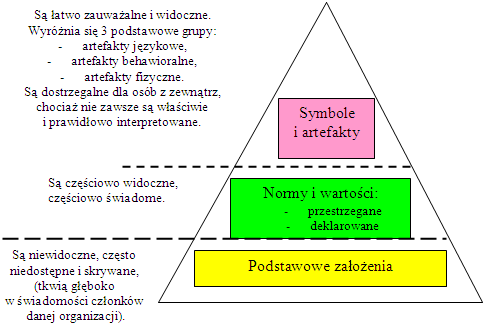
\includegraphics[scale=0.5]{assets/poziomy}
\begin{itemize}
	\item Symbole i artefakty
	\begin{itemize}
		\item Charakterystyka: widoczne, świadome ale wymagające interpretacji
		\item Przejawy: symbole pojęciowe (anegdoty, legendy)
		\item Przejawy: symbole behawioralne (zwyczaje)
		\item Przejawy: symbole materialne (ubiór, budynki)
	\end{itemize}
	\item Uznane normy i wartości
	\begin{itemize}
		\item Charakterystyka: częściowo widoczne i czasowo swiadome
		\item Przejawy: maksymy, ideologie, zakazy, nakazy, hierarchi, wartości
	\end{itemize}
	\item Podstawowe założenia
	\begin{itemize}
		\item Charakterystyka: niewidoczne, nieświadome
		\item Przejawy: pojmowanie otoczenia, autorytety, wizje znaczenie pracy	
	\end{itemize}
\end{itemize}

\noindent Artefakty:
\begin{itemize}
	\item widoczne przejawy kultury organizacyjnej, do której zalicza się:
	\begin{itemize}
		\item artefakty fizyczne -- wytowory materialne danej kultury
		\item artefakty behawioralne -- ceremonie, rytuały
		\item artefakty językowe -- specyficzne język organizacji; mity + legendy
	\end{itemize}
\end{itemize}

\noindent Cztery typy kultury organizacyjnej -- wg Rogera Harrisona
\begin{enumerate}
	\item kultura władzy (Zeusa) -- najwyższą wartością są pieniądze i status. Mamy do czynienia z silną włądzą
	\begin{itemize}
		\item znajomości
		\item kontorla procesu i efektu -- totalna
	\end{itemize}
	\item Kulutra roli (Apolla) -- dużą wagę przywiązuje się do funkcji, stanowiska czy specjalizacji. Przykładem jest biurokracja w urzędach czy dużych firmach monopolistycznych
	\begin{itemize}
		\item kwalifikacje, prawo
		\item kontrola procesu
	\end{itemize}
	\item Kultura zadania (Ateny) -- działania są nastawione na rozwiązywanie problemóœ. Praca w zespołach, zdecentralizowane zarządzanie, elastyczność. W kulturze zadania interesy jednostki mogą być poświęcone dla utrzymania istnienia zespołu
	\begin{itemize}
		\item kompetencje
		\item kontrola efektu
	\end{itemize}
	\item Kultura osoby (Dionizosa) -- podstawowym cele jest służenie jednostkom, działanie organizacji jest podporządkowane potrzebom jej członków. Przykład to zespół wysoko wykwalifikowanych specjalistów.
	\begin{itemize}
		\item Wolność
		\item zewnętrzna kontrola efektu
	\end{itemize}
\end{enumerate}

\section{30 IV 2015 (Opolski) TODO}
\section{5 V 2015 (Górski) TODO}

\section{7 V 2015 (Oposki)}

\noindent Wzory zachowań indywidualnych konieczne do funkcjonowania i efektywności organizacji
\begin{itemize}
	\item Włączenie się do systemu i pozostawanie w nim
	\begin{itemize}
		\item rekrutacja
		\item niska absencja
		\item mała płynność kadr
	\end{itemize}
	\item Niezawodność zachowań: pełnienie ról w systemie
	\begin{itemize}
		\item wypełnianie lub przekraczanie ilościowych norm wykonania zadań
		\item wypełnianie lub przekraczanie jakościowych norm wykonania zadań
	\end{itemize}
	\item Zachowania innowacyjne i spontaniczne: wykonywanie zadań wykraczające poza wymagania roli związane z wypełnieniem danej funkcji w organizacji
	\begin{itemize}
		\item działania kooperujące
		\item działania chroniące system lub podsystem
		\item twórcze sugestie dotyczące ulepszania organizacji
		\item samokształcenie w związku z dodatkowymi obowiązakami w organizacji
		\item stwarzania korzystnej dla organizacji atmosfery w środowisku zewnętrznym
	\end{itemize}
\end{itemize}

\noindent Wzory motywacyjne będące podstawą wytwarzania różnych rodzajów wymaganych zachowań
\begin{itemize}
	\item podporządkowanie się prawom
	\begin{itemize}
		\item zapewnienie akceptacji nakazów roli i organizacyjnych środków kontroli, przez powołanie się na ich legalność. Podejście na oparte na przestrzeganiu przepisów, charakterystyczne dla prostej teorii mechanistycznej
	\end{itemize}
	\item zastosowanie nagród -- czyli satysfakcji instrumentalnych, w celu wywołania pożądanych zachowań. Podejście charakterystyczne dla zmodyfikowanej teorii mechanicznej
	\begin{itemize}
		\item Nagrody systemy
		\begin{itemize}
			\item uzyskiwane dzięki przynależności do systemu lub na podstawie czasu pozostawania w nim, takie jak zasiłki, podwyżki pokrywające wzrost kosztów utrzymania i inne świadczenia obejmujące całą załogę
		\end{itemize}
		\item nagrody indywidualne
		\begin{itemize}
			\item takie jak premie i awanse, oparte na zasługach indywidualnych
		\end{itemize}
		\item instrumentalna identyfikacja z przywódcami
		\begin{itemize}
			\item zwolennicy pragną uzyskać aprobatę swoich przywódców
		\end{itemize}
		\item potrzeba afiliacji
		\begin{itemize}
			\item pragnienie uzyskania aprobaty grupy
		\end{itemize}
	\end{itemize}
	\item zinternalizowany wzór samostanowienia i autoekspresji
	\begin{itemize}
		\item satysfakcja płynąca z wykorzystania i ujawnienia talentów i zdolności
		\item występuje w organizacjach, gdzie pracownik nie jest wciskany w role i konkretne ramy
	\end{itemize}
	\item zinternalizowane wartości i obraz "Ja"
	\begin{itemize}
		\item cele lub podcele organizacji uznane są za odbicia wartości i obrazu "Ja"
	\end{itemize}
\end{itemize}

\noindent Warunki, od których uzależniona jest aktywizacja wzoru A -- "podporządkowanie się prawom"

\begin{itemize}
	\item warunki obiektywne
	\begin{itemize}
		\item wykorzystanie odpowiednich symboli zwierzchnistwa
		\item jasność legalnych norm i wymagań
		\item zastosowanie specyficznych kar
		\item wuswanie nonkonformistów
	\end{itemize}
	\item zmienne pośredniczące  o charakterze psychologicznym
	\begin{itemize}
		\item rozoznanie i akceptacja
		\item nie ma subiektywnej dwuznaczności dopuszczającej interpretację życzeniową
		\item indywidualne obawy przez "przyłapaniem"
		\item pragnienie, aby pozostać w systmeie: system wpływa na sposób bycia
	\end{itemize}
	\item Wyniki -- skutki
	\begin{itemize}
		\item ilość i jakośc pracy utrzymuję się na minimalnym dającym się akceptować poziomie
		\item może obniżyć się absencja
		\item może zwiększyć płynność kadr
		\item niekorzystny wpływ na zachowania innowacyjne i inne wykraczające poza obowiązki
	\end{itemize}
\end{itemize}

\noindent warunki wpływające na zastosowanie indywidualnych nagród pienięznych
\begin{itemize}
	\item warunki obiektywne
	\begin{itemize}
		\item wielkość nagrody za wysiłek indywidualny
		\item bezpośredność
		\item stałość nagród
	\end{itemize}
	\item Wyniki -- skutki
	\begin{itemize}
		\item może zmniejszyć płynność kadr
		\item pewne ograniczenie absencji
		\item możiwy wzrost produktywnośći. Niekonieczny wzrost zachowań kooperujących lub ochraniających. Możliwy wzrost sugestii twórczych
	\end{itemize}	
\end{itemize}

\noindent Nagrody systemowe
\begin{itemize}
	\item warunki obiektywne
	\begin{itemize}
		\item dostępny dla jednostki alternatywny system
		\item bezpośredniość
		\item stałość nagród
	\end{itemize}
	\item Wyniki -- skutki
	\begin{itemize}
		\item zmniejszenie płynności kadr
		\item pewne zmienjszenie absencji. 
		\item minimalny poziom jakościowy i ilościowy pełnienia ról
		\item brak tóœrczego wkładu do org.
		\item  stwarzanie korzystnej atmosfery w środowisku zewnętrznym
	\end{itemize}	
\end{itemize}

\noindent Aprobaty grupy koleżeńskiej
\begin{itemize}
	\item warunki obiektywne
	\begin{itemize}
		\item spójność grupy
	\end{itemize}
	\item zmianne pośredniczące  o charakterze psychologicznym
	\begin{itemize}
		\item przywiązanie jednostki do grupy
	\end{itemize}	
	\item Wyniki -- skutki
	\begin{itemize}
		\item zmienjszenie absencji i płynności kadr
		\item możliwy wzrost lub spadek produktywności
		\item niekonieczny związek z zachowaniami wykraczającymi poza obowiązki
	\end{itemize}	
\end{itemize}

\noindent warunki wpływające na zaistnienie talentów i zdolności samostanowienia jako sposobu motywowania
\begin{itemize}
	\item warunki obiektywne
	\begin{itemize}
		\item Złożoność zajęcia i wymagane kwalifikacje
		\item odpowiedzialność i autonomia związana ze stanowiskiem
		\item Możłiwość innych zajęć
	\end{itemize}
	\item Wyniki -- skutki
	\begin{itemize}
		\item niekonieczny związek z płynnością kadr
		\item zmniejszenie absencji
		\item wysoka produktywność
		\item pewien wzrost działań kooperyjących, lecz ogólnie mały związek z zachowaniami wykraczającymi poza obowiązki
	\end{itemize}	
\end{itemize}

\noindent Warunki wpływające na wykorzystanie zinternalizowanych wartości i obrazu własnego "Ja" jako sposobu motywowania
\begin{itemize}
	\item warunki obiektywne
	\begin{itemize}
		\item ryzykowność celów organizacji
		\item cele organizacji są wyrazem wartości kulturowych
		\item przywódca organizacji jest wzorem
		\item udział w podejmowaniu decyzji
		\item udział w nagrodach
	\end{itemize}
	\item Wyniki -- skutki
	\begin{itemize}
		\item zmniejszenie płynności kadr i absencji
		\item zwiększona produktywność
		\item zachowanie spontaniczne i innowacyjne
	\end{itemize}	
\end{itemize}

\chapter{Temat 9 Kapitał ludzki, intelektualny i społeczny organizacji}

\section{7 V 2015 (Opolski)}

\section{12 V 2015 (Górski) }

\medskip
	
\end{document}
